\documentclass[12pt,a4paper,notitlepage]{report}
\usepackage[utf8]{inputenc}
\usepackage{cite}
\usepackage{etoolbox}
\usepackage{listings}
\usepackage{graphicx}
\usepackage{subcaption}
\usepackage{amsmath}
\usepackage{titlesec}
\usepackage[nottoc, notlof]{tocbibind}
\usepackage{pgfplots}
\usepackage{siunitx}
\usepackage{multirow}
% might need later, for diagrams
%\usepackage{tikz}
%\usetikzlibrary{arrows,shadows}
%\usepackage{pgf-umlsd}

\def\checkmark{\tikz\fill[scale=0.4](0,.35) -- (.25,0) -- (1,.7) -- (.25,.15) -- cycle;}

%%%%%%%% Bibliografi %%%%%%%%%%%%%%%%%%%%%%%%%%%%%%%%%
%% Ändrar namnet på referens headern
\renewcommand\bibname{ References}
%%%%%%%%%%%%%%%%%%%%%%%%%%%%%%%%%%%%%%%%%%%%%%%%%%%%%%

%\titleformat{\chapter}[display]
%  {\normalfont\bfseries}{}{0pt}{\Large}

\titleformat{\chapter}[display]
 {\normalfont\bfseries}{}{0pt}{\Large \thechapter }

%%%%%%%%%%%%%%%%% Start document %%%%%%%%%%%%%%%%%%%%%
\begin{document}
\pagenumbering{roman}

\title{Digitalization of Visual Acuity Testing}
\author{Anders Ohlsson\\Christian Johansson\\Svante Nilsson}
\maketitle

\begin{abstract}
Digitalization of Visual Acuity Testing is a project about digitally displaying and manipulating optician's eye charts. The charts are displayed on a digital screen with a lightweight server running on a Raspberry Pi and controlled over a wireless network via an Android tablet. 
%%This solves several problems related to the distance from the patient to the chart, while also providing more ways for the optician to tailor the examination to the patient.
This allows the charts to adapt when placed at different distances from the patient, while also allowing the optometrist to tailor the examination to the patient by switching between multiple sheet designs and specialized sets of characters. 
The Digitalization of Visual Acuity Testing project has improved upon a proof-of-concept system that has been used at the Uppsala University Hospital to test whether or not digital screens are a viable alternative to physical charts. The project fulfils its goals and has performed well under testing, but more testing is needed to make sure it meets the demands of practising optometrists.
\end{abstract}
\renewcommand{\abstractname}{Sammanfattning}
\begin{abstract}
Digitalization of Visual Acuity Testing är ett projekt om att visa och manipulera syntavlor digitalt. Syntavlorna visas på en bildskärm kopplad till en enkel server som är installerad på en Raspberry Pi och kan styras över ett trådlöst nätverk med hjälp av en Androidsurfplatta. Eftersom tavlorna är digitala kan de anpassas till avståndet mellan patienten och tavlan, samtidigt som de låter en optiker anpassa synundersökningen till patienten genom att tillåta snabbt byte av syntavlans layout och symboler. Projektet bygger på ett testsystem som har använts vid Akademiska Sjukhuset för att undersöka ifall digitala skärmar är ett passande alternativ till trykta syntavlor. Digitalization of Visual Acuity Testing har uppfyllt sina mål och har presterat väl i tester, men mer tester måste genomföras för att se till att det upfyller alla krav en optiker skulle kunna ha på projektet.
\end{abstract}
\renewcommand\thechapter{ }
\tableofcontents*
\listoffigures
\clearpage

\renewcommand\thechapter{\arabic{chapter}}
\pagenumbering{arabic}
\setcounter{page}{1}
\chapter{ Introduction}
\section{Background}
The standard way for an optician to measure a patients visual acuity is to use charts printed with rows of continuously smaller symbols called optotypes~(fig.~\ref{fig:optotypes_example1}), most often normal Latin letters. The patient reads the symbols on the chart in order until he or she can no longer correctly identify them. Each row on the chart has a pre-calculated number printed beside it, which will help the optician determine which lenses the patient should try next.

\begin{figure}[ht!]
\centering
\begin{subfigure}{.3\textwidth}
  \centering
  
\includegraphics[width=.4\linewidth]{images/landholt_c_optotype.png}
  \caption{Landholt C}
\end{subfigure}%
\begin{subfigure}{.3\textwidth}
  \centering
  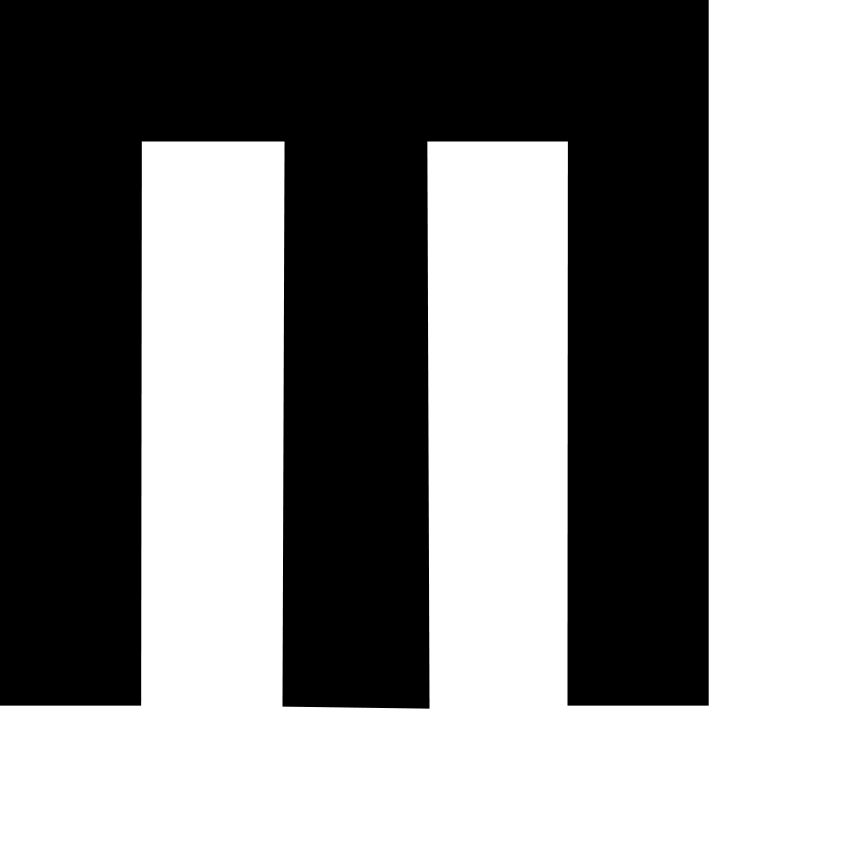
\includegraphics[width=.4\linewidth]{images/tumbling_e_optotype.png}
  \caption{Tumbling E}
\end{subfigure}
\begin{subfigure}{.3\textwidth}
  \centering
  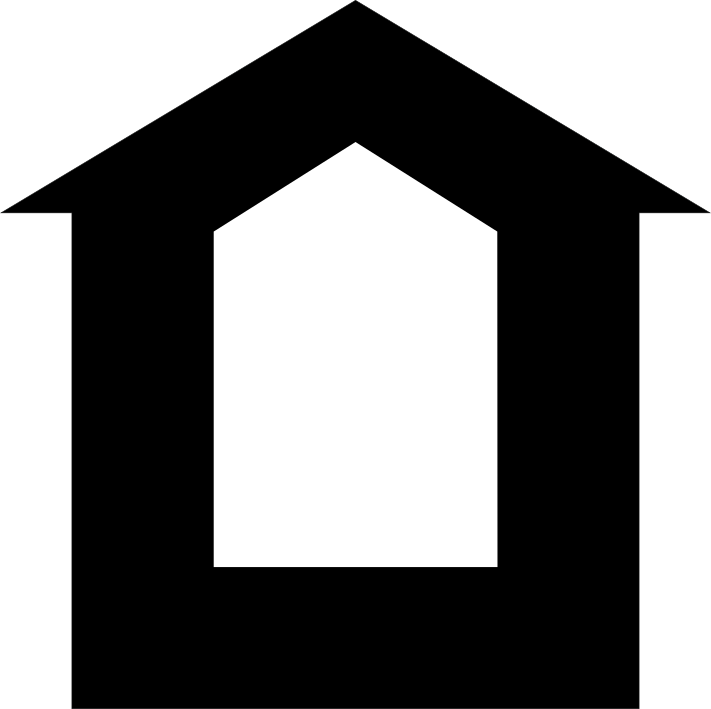
\includegraphics[width=.4\linewidth]{images/lea_optotype.png}
  \caption{LEA}
\end{subfigure}
\caption{Some example optotypes}
\label{fig:optotypes_example1}
\end{figure}

These numbers have been calculated from a set of standardized conditions~\cite{Bailey}. For example there must be adequate lighting in the room so the patient can read the letters, but more importantly the charts are meant to be placed a fixed distance from the patient. For most charts, this distance is six meters. 

These conditions cannot always be met. Examination rooms are not always large enough to take measurements from six meters away for example. In those cases, the reference numbers on the sheet are no longer accurate and the optician has to compensate manually~\cite{PGSoderberg}. If the standardized conditions cannot be met it can lead to irregularities or faulty measurements in some tests.

There are also several different variations on these eye charts. Different sets of optotypes, ranging from different subsets of Latin letters to more abstract symbols, have been developed for different types of patients, such as those who are analphabetic, or for small children. The layout of these charts also have variations, from the classic Snellen chart~(fig.~\ref{fig:snellen_chart1}) that was developed in the 19th century, to the more modern ETDRS (Early Treatment Diabetic Retinopathy Study) chart~(fig.~\ref{fig:etdrs_chart1}).


In a field so dependent on visual aids and equipment, it's easy to see that there are several possibilities for improvement and expansion. Modern technology can be used to improve these tests, and digitalization can simplify the way opticians work with diagrams.

\begin{figure}[ht!]
\centering
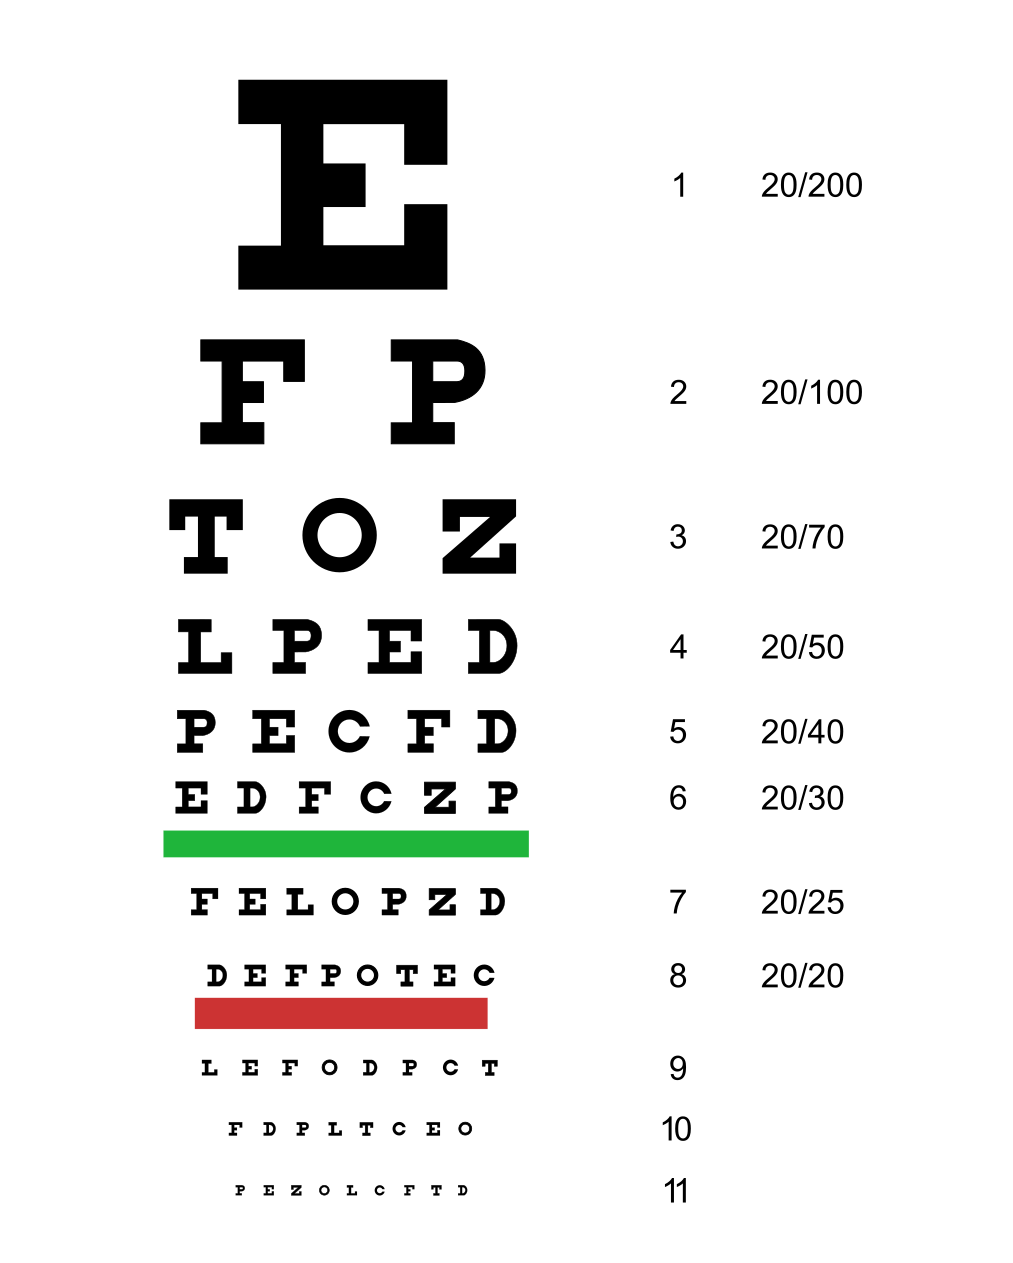
\includegraphics[width=110mm]{images/Snellen_chart.png}
\caption{The Snellen chart (Source: http://en.wikipedia.org/wiki/Snellen chart\cite{img_snellen}).} \label{fig:snellen_chart1}
\end{figure} 

\begin{figure}[ht!]
\centering
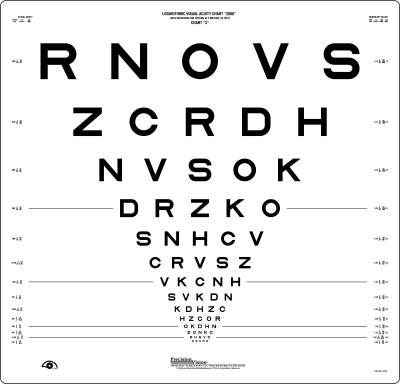
\includegraphics[width=120mm]{images/etdrs_chart.jpg}
\caption{The ETDRS chart, used with permission from Precision Vision \\ (Source: http://precision-vision.com/)\label{fig:etdrs_chart1}}
\end{figure} 

\section{Purpose}
Having efficient and accurate systems is important in a medical environment, especially in a medical environment that handles tests where inaccurate or false results in some cases can cause accidents. Therefore it is important to have a well-built system that mitigates these problems. With the help of Professor Per Söderberg as our expert in the field of ophthalmology we will try to create a system that will act as a prototype for further future work. 

Accuracy is not the only important aspect to think of when implementing a system. It is also important to think about expanding and improving on how the system can be used. To introduce new functionality that will make the life of the system's user a lot more simple and efficient is one of those important improvements. 

These are a few of the aspects that we will to build a system around. A simple system that implements digital eye charts has already been built by professor Söderberg, though that system is not as sophisticated or expendable as needed. We base some of our system's content upon how this other system is built. Mostly this will be using the layouts of the charts already created since those charts have been shown to work. 

Using this other system as a basis for our own we build a system that:

\begin{itemize}
	\item Has an application for the Android tablet with an improved user interface, both aesthetically and functionally.
	\item Controls a server that renders the eye charts on a screen over WiFi using the Android tablet.
	\item Can alter the scale of the rendered symbols so that the patient can be closer or further away from the screen.
	\item Has functionality to tailor the testing process by, among other things, changing the sets of symbols displayed or removing clutter from the charts.
\end{itemize}

\section{Motivation}
Building upon what is said in the last section we need to find a clear motivation on why this should be done. A few things can be found in the working environment of the optician. Determining visual acuity is a very labor- and equipment-intensive process. It is a lot of manual labor with much time wasted when setting up and changing the equipment used. This work-load is also increasing drastically with time. More and more people are experiencing eye problems, at all ages and in many cultures. \cite{vision_loss} With more people needing to test their visual acuity, faster and more efficient methods needs to be used. 

Another fact is that physical eye charts are not as accurate as they should be for accurate measurements. They are also big in size and static, static in this context because they are fixed and cannot be changed. Because the handling of printed charts is slow and not as accurate as needed there exists a need for improvement. 

A digital eye chart has increased functionality, accuracy and efficiency which are all important aspects to approve upon. A digitalization also gives the user a greater possibility for extending the usage of the system.

\section{Issues}
There are several technical problems that we need to solve. We need to find a suitable computer system that will act as the server, its job being storing and presenting the desired images to the screen. Our current plan is to use a Raspberry Pi, since it is a cheap and compact alternative to a full-size computer that is more than powerful enough for our purposes. Though, since the Raspberry Pi's CPU is running on an ARM-architecture there will be a few compatibility problems. For example, the newly redesigned Java graphics library JavaFX, that is going to replace the older Swing library, has very bad support for ARM. Not being able to use the latest features can create problems in the future when some things get deprecated. If Java Swing would happen to become deprecated it should not be too difficult to transfer the code to a hopefully compatible Java FX version.  

Designing the Android app for the tablet will also bring technical problems, both from the limitations of portable computers, and making our software adaptable enough to work on as many brands of tablets as possible. For example, the symbols we are to present are stored in the .SVG (Scalable Vector Graphics) format, which is not natively supported on Android. Because of this we must find and work with a licensed third-party software library to render them. 

Finally, we have the issue of networking. A lot can go wrong when trying to control a program over a network and also trying to have the response be fast and accurate. Any problems between the controller and the server will make actions seem slow and inconsistent. It can be even worse when working on a wireless network as in our case. This is an equally important problem as the other ones, but there exists several great technologies helping to prevent these kind of issues that will be a great help to us. 

%\section{Ethical considerations}
%Our ethical obligations with this project is providing a functional and stable product. If our system does not perform to specification, a lot of patients could get erroneous measurements during testing, costing a lot of time and money to correct. This is very important to think about since we are dealing with treatment of people. All of this has to be considered even if the final results will not be used clinically.

\chapter{ Problem Description}
\section{Problem}
\subsection{Gammalt, bakas in i det ovan (Ta bort denna subsection)}
%The problem with today's visual acuity testing charts are that they are very clumsy to work with. The charts are printed and contains only one static selection of symbols, also called optotypes. This could be optotypes for people with the ability to read or an 'E' shape rotated in different directions which allows children who are unable to read, or illiterate people, to identify which symbol they see. These static charts are also designed to be viewed from one specific distance. This causes problems when dealing with environments that are too small, for example erroneous measurements. 
There are several weaknesses with visual acuity testing today that we have worked on improving. Physical charts are often large and cumbersome to switch if the patient needs a chart with another type of optotypes. Since they are also designed for standardized distances and testing conditions, an optician needs to manually compensate for any deviations from the standard. 

There are also other problems with using standardized charts, such as older patients getting lost among the columns and rows, and other patients memorizing the rows of letters to cheat. Giving the optician the option of using randomly generated charts and easily switching between specialized chart layouts can greatly increase the speed and accuracy of testing.

Another problem we faced is designing a user interface that can give the optician easy access to these specialized charts and layouts. An intuitive design so that it is easy to learn, and a user friendly design so that users don't accidentally make unintentional or irreversible changes.

\subsection{Nytt, behålls, bara denna rubrik tas bort när det gamla är fixat \\ se över den här texten så det inte blir nya problem}
We want to create a system that allows opticians to quickly prepare and perform an eye examination using a chart displayed on a monitor controlled by an Android device. 
----------------SKRIV MER HÄR!!!!!!!!!----------- (ELLER SKRIV OM!!!!)

\section{Delimitations}
Due to limits in time and manpower, this project is not intended to result in a complete working system to be used clinically, but rather a working prototype that can be used to evaluate digital visual acuity charts. To complete the project on time, as much as possible of Java's and Android's built-in libraries will be used in order to avoid recreating code that already exists, thus saving time. Neither Java nor Android include libraries for rendering SVG-files and third party libraries will be used instead.

%Though as SVG-files are going to be used for the rendering of optotypes and neither Java or Android supports it natively third-party libraries will be used.

We will not evaluate a digital screen's effect on the eye compared to a physical chart nor analyze why a chart should have the layouts it has. As the visual acuity charts are made after a very strict specification, no new chart layouts will be made. Any new chart we would create would be considered useless without backing research and they could be misleading and misused by future users that in the end, could result in patients getting an inaccurate result.

No security features, such as encrypted network traffic or protection against several users connecting to the same server at the same time, will be implemented. Instead, this is left to the user to make sure that a secure network is used. Since there is no patient data or other private information being transmitted or stored we don't see the need for secure connections in this project.

No automatic update system will be included, instead the user will have to manually update both the Android application and the server. Automatic updating was not a core feature, and could therefore be saved for future work.

\section{Requirements}
%For this project to be considered successful, the system must be able to display the chart chosen by the user. This means that the user have to be able to control which chart type to display on the monitor from an Android device. The types of charts that should be included are the four Axanivis charts, the upper, the lower, the one line and the single optotype chart. The user also has to be able to choose if the current chart should use the Sloan, Tumbling E, HVOT or LEA optotypes.

For this project to be considered successful, the system must be able to display the chart chosen by the user. This means that the user have to be able to control which chart type to display on the monitor from an Android device. The types of charts that should be included are the four Axanivis charts (fig. \ref{fig:axanivis}), which is a project under development by P.G. Söderberg \cite{PGSoderbergOral}.

\begin{figure}[ht!]
\centering
\begin{subfigure}{.5\textwidth}
  \centering
  %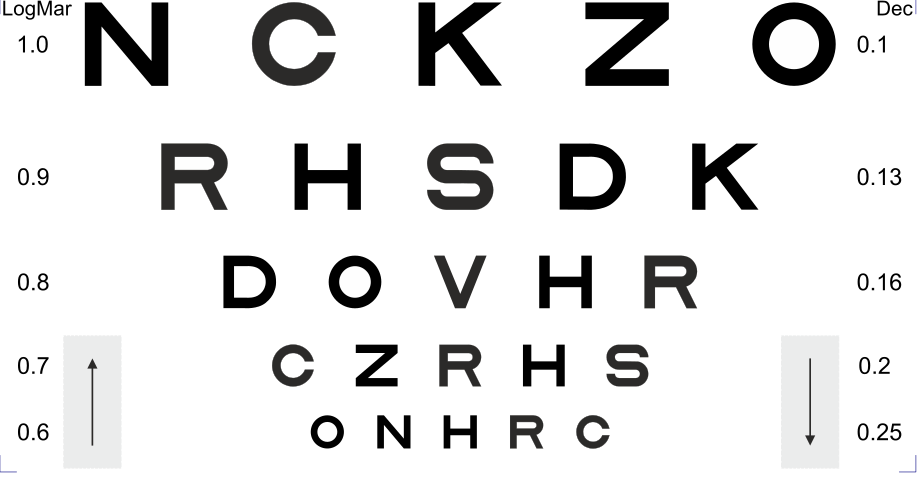
\includegraphics[width=.5\linewidth]{images/etdrs_top.png}
  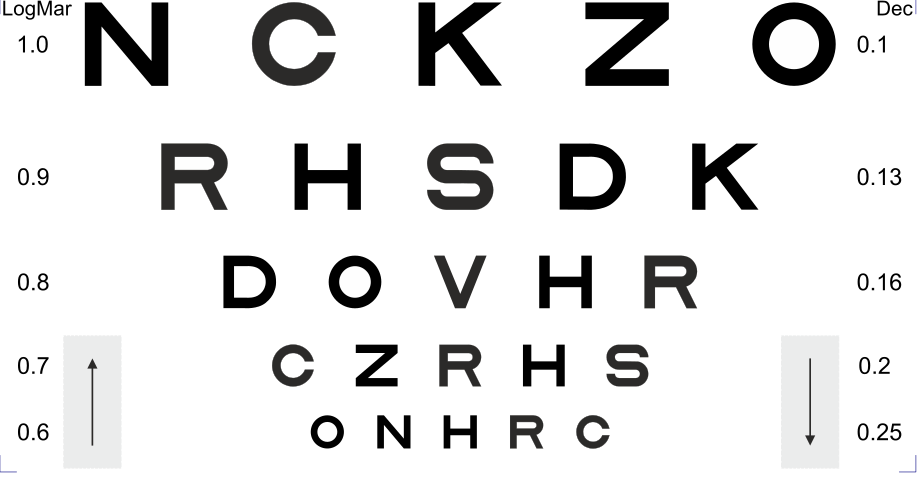
\includegraphics[width=50mm]{images/etdrs_top.png}
  \label{fig:etdrs_upper1}
\end{subfigure}%
\begin{subfigure}{.5\textwidth}
  \centering
  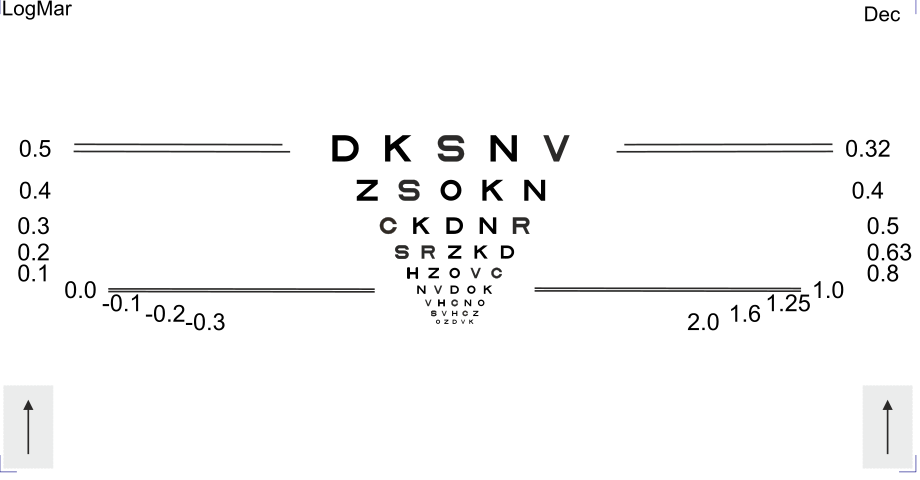
\includegraphics[width=50mm]{images/etdrs_bottom.png}
  \label{fig:etdrs_lower1}
\end{subfigure}
\begin{subfigure}{.4\textwidth}
	\centering
	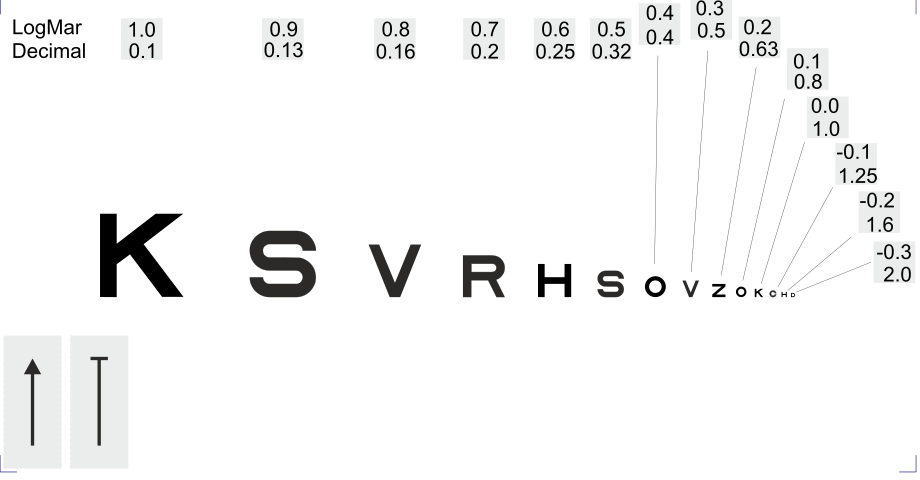
\includegraphics[width=50mm]{images/etdrs_one_line.png}
\end{subfigure}
\begin{subfigure}{.4\textwidth}
	\centering
	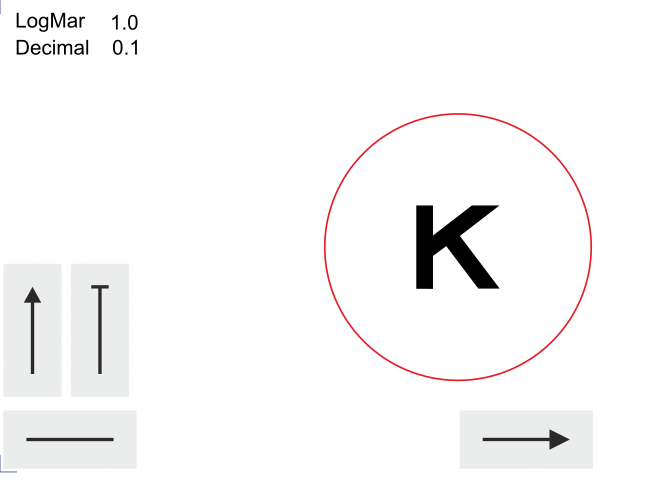
\includegraphics[width=50mm]{images/etdrs_single.png}
\end{subfigure}
\caption{The four Axanvis charts}
\label{fig:axanivis}
\end{figure}


The user also have to be able to choose if the current chart should use the Sloan, Tumbling E, HVOT or LEA optotypes (fig. \ref{fig:optotypes_example1}). The Sloan and HVOT optoypes consists of a different sets of letters, the Tumbling E consists of the letter E rotated in different angles and LEA is a set of custom symbols. \cite{Colenbrander}

\begin{figure}[ht!]
\centering
\begin{subfigure}{.3\textwidth}
  \centering
  
\includegraphics[width=.4\linewidth]{images/landholt_c_optotype.png}
  \caption{A Sloan C}
  \label{fig:landholt_c1}
\end{subfigure}%
\begin{subfigure}{.3\textwidth}
  \centering
  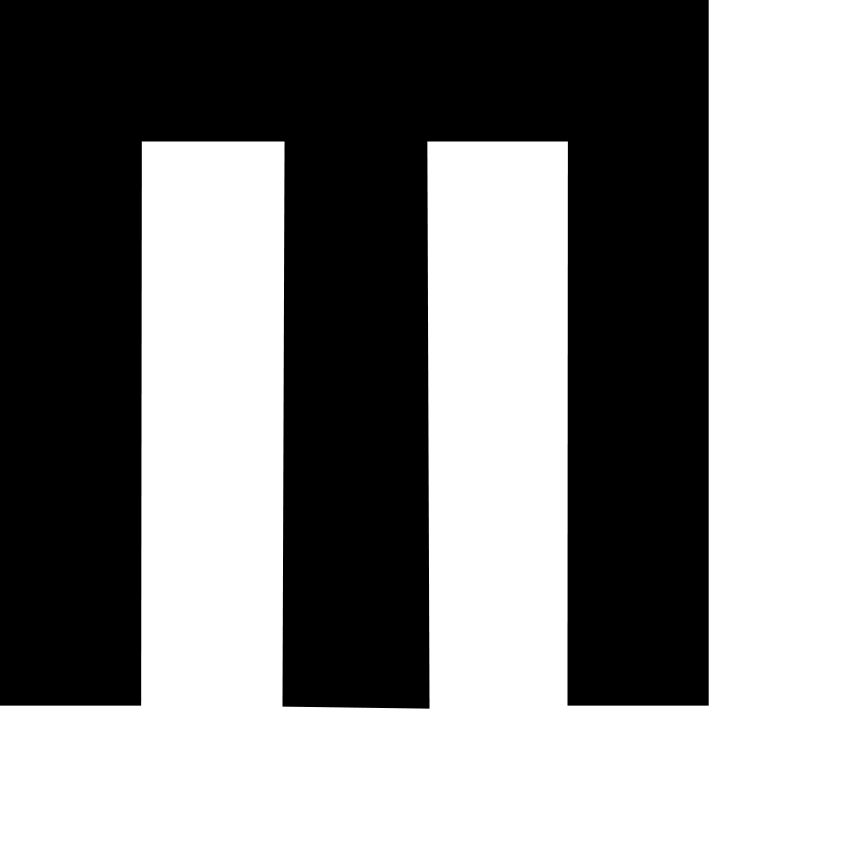
\includegraphics[width=.4\linewidth]{images/tumbling_e_optotype.png}
  \caption{A Tumbling E}
  \label{fig:tumbling_e1}
\end{subfigure}
\begin{subfigure}{.3\textwidth}
  \centering
  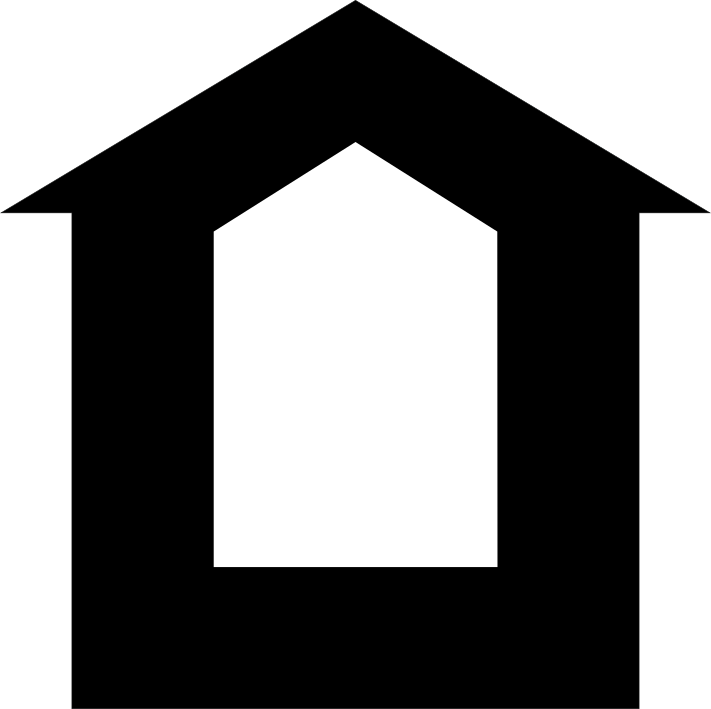
\includegraphics[width=.4\linewidth]{images/lea_optotype.png}
  \caption{A LEA House}
  \label{fig:lea1}
\end{subfigure}
\caption{Some example optotypes}
\label{fig:optotypes_example1}
\end{figure}

It is very important that the chart on the monitor displays all optotypes with the correct sizes and positions. In order to do this, the user must to be able control the distance from which the patient is watching the monitor. It is also very important that the correct sizes, in LogMAR (Logarithmic of the Minimum Angle of Resolution), which is a logarithmic unit of measurement dependant on the view angle of a patient \cite{Bailey}, is displayed on the Android device.

The intended user for this system should have all the necessary knowledge and education on how to perform an eye examination. The user should not need any more than basic knowledge about an Android device, such as being able to start the device, connect to a wireless network, start an application and how to perform simple Android gestures. This does not mean that it has to be easy to install and set up, though it is a goal for future expansion. 

The Android application should follow the Android design principles set up by Google \cite{android_design}. This makes the application behave similar to other Android applications which will result in users already familiar with Android feel familiar to this application as well.

The system should also allow for automatic server detection so that users don't have to manually connect by entering IP addresses. This allows a quick and easy way to connect to a server. In order for the server detection to be considered working properly, it should detect a server on a stable network at least 90\% of the time. With a success rate of 90\%, it would be very uncommon to fail the detection twice in a row, while keeping the scanning time relatively low.

As this project only aims for a working prototype of the system, it is very important that it is easy to continue the development and add more features without rewriting large parts of the code.

\section{Evaluation \label{sec:evaluation}}
In order to evaluate if all requirements have been met, the system will undergo four tests. The goal of the first test is to make sure that the user actually can choose a specific chart with specific optotypes to be viewed from a specific distance. This is done by the developers going through all charts, with all types of optotypes and setting the distance for each one of them. To achieve this, table \ref{tab:test1_empty} is used to systematically walk through every setting.

The second test is to make sure that the optotypes have the correct sizes on the monitor. This test will be done by calculating the expected sizes of the optotypes in centimeters for different screen sizes with the help of Matlab. The calculated sizes will then be compared to the sizes output by the system and see if they match. If this is a match, the optotypes will be measured by a physical measurement tool in order to make sure that they have the calculated size when they are displayed on the monitor. The physical measuring is required to make sure that the system works as intended in practice and not only in theory.

The third test will determine how user friendly the system is. This will be done by letting a user with no previous knowledge of the system, attempt to connect to a server and perform some basic tasks like setting a specific chart with a specific optotype or setting a specific distance (App. \ref{app:usability}). If the user testing has no previous knowledge of visual acuity charts, a brief explanation will be given so that the test doesn't fail because the user, for example, doesn't know what "HVOT" is. Once the test is done, the user will provide feedback pointing out possible faults in our design. This feedback will then be used to improve the design. If the user can perform the entire test without help, the test is considered successful.

The last test is a quantitative test to see how well the server detection performs. The test involves the Android application trying to detect a server on a stable WiFi a 100 times and see how many times the server was detected. This test can be done several times and the average number of detection's in a 100 tries will determine its success rate. Testing the system on anything other than a stable WiFi is unnecessary as it is only intended to work on a stable local network.

\section{Related work}

\subsection{Visual acuity charts}
Several different versions of visual acuity chart exist today. The ETDRS (Early Treatment Diabetic Retinopathy Study) chart is the most commonly used today and is an improvement to the older \textit{Snellen chart}(fig. \ref{fig:snellen_chart1}, page \pageref{fig:snellen_chart1}). The ETDRS chart was designed and developed by Ferris et al \cite{Ferris}, based on the work of Bailey and Lovie \cite{Bailey}. 

%\begin{figure}[ht!]
%\centering
%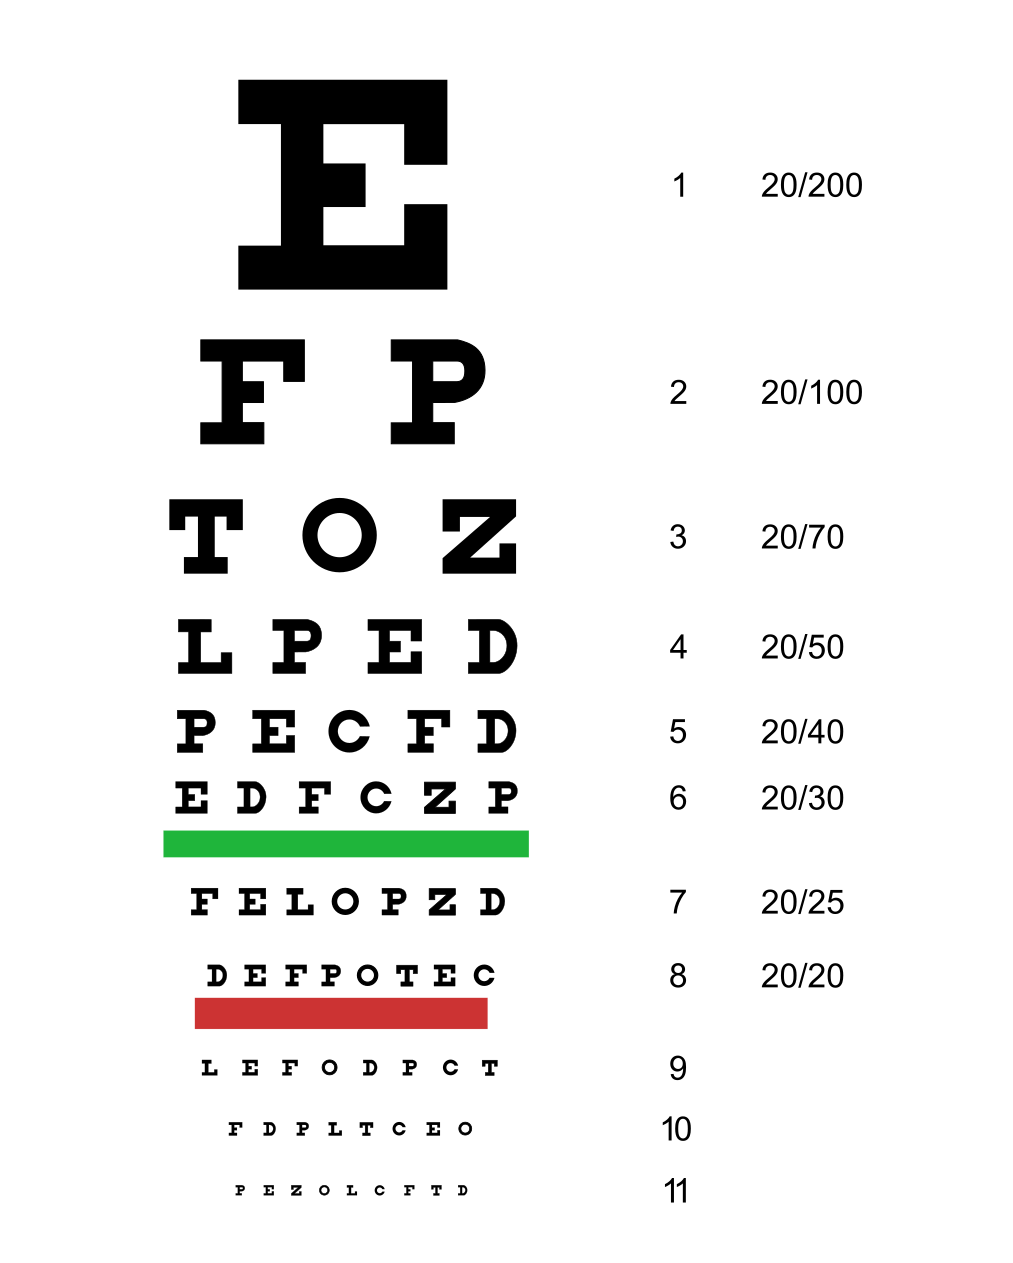
\includegraphics[width=60mm]{images/Snellen_chart.png}
%\caption{The Snellen chart (Source: http://en.wikipedia.org/wiki/Snellen chart\cite{img_snellen}).} \label{fig:snellen_chart}
%\end{figure} 


\subsection{Digital visual acuity charts}
Digital Eye Chart \cite{digitaleyechart} and iChartPlus \cite{ichartplus} are two applications supposed to display a visual acuity chart on a digital screen. Both applications are computer applications, which requires the computer to be connected to the screen. The companies behind the products provide very little information and the exact specifications of the charts are not available.

\subsection{Media streaming devices}
Several media streaming devices exists that allow digital content to be received and displayed on a connected screen. Examples of such devices are Chromecast \cite{chromecast} and Apple TV \cite{appletv} which you can plug into a TV and allows you to view images or watch movies that are stored on your phone or computer. Both applications also allows developers to develop their own applications to display custom content but requires the developer to enter an agreement with respective company.


%There exists today several companies that have taken on the task of digitalizing the usage of eye charts.
%
%\subsubsection{Chromecast and Apple TV}
%The Chromecast \cite{chromecast} and Apple TV \cite{appletv} are small devices which are plugged into a TV and enables mobile phones and tablets to stream media to them. The devices are small and easy to handle and a lot of applications support streaming to them. The Chromecast is specifically made for Android devices and Apple TV for iOS device, but they both support each other.
%
%\subsubsection{Digital Eye Chart}
% Digital Eye Chart \cite{digitaleyechart} is a visual acuity testing program that attempts to solve the problem of having several charts by using a monitor instead. The user can then, with the help of a computer, change the symbols on the chart and even generate a random chart. 
%
%\subsubsection{iChart+}
%iChartPlus \cite{ichartplus} is another program which is similar to Digital Eye Chart but also have an adjustable viewing distance. 
%
%\subsubsection{AxAnIvIs}
%AxAnIvIs is a prototype that is currently under testing at Uppsala University Hospital. The project attempts to improve on how we perform visual acuity tests by digitalizing them. It adds more types of charts than the standard physical ones that exists today. The system uses a webbrowser running on an Android tablet that is connected to a screen. A library of vector graphic files are displayed in the webbrowser. These files contains the different charts as well as some other specialized tools. Currently the Android tablet has to be held in a fixed position in the examination room, restrained by the cable going to the screen. The charts used are fixed and not very easily changed, which makes it very hard to try out new techniques and methods of measuring.
%
%\subsubsection{Our project}
%Most of the before mentioned systems have some form of negative side that we try to improve on, mostly problems about high cost and difficulties with extending the software. We are different with that we want to create a system that is cheap, easy to understand and easy to maintain. Creating a system that have all the previously mentioned sides is one of the goals we have. Another important goal is creating a system that really is speacialized on measurements of visual acuity. All these points are important to give the users the best experience.

\chapter{ Visual Acuity Testing}
\section{Visual Acuity}
The measurement of a persons visual acuity has an important constraint that needs to be followed. This constraint is the fact that our eyes works best physiologically from greater distances. On the other hand, at shorter distances our eyes tend to make what we see look unfocused. To make up for this shift in focus a minimum testing distance has to be enforced to ensure that the shift in focus stays as small as possible. This distance has by scientific research been set to be six meters.

\subsection{Measurement distance}
The specific distance of six meters is derived from how our eyes bend light. From that distance or greater the rays of light entering our eyes are nearly parallel to each other, parallel enough to make it unnoticeable. It is important that the rays of light that hit the eyes are parallel because then the light hits a more focused area in the back of the eyes. This happens because of the convex shape of the eye's lens. A convex shaped lens focuses parallel light onto the focal point. Since a convex lens focuses parallel light to a focal point a concave lens instead spreads light coming from a focal point to parallel rays. Combining these two type of lenses we can create a more focused light. 

\subsection{Defocus correction}
To make up for the shift in focus a suitable lens is put in front of the eye at about the distance that you would wear glasses. The type of lens mostly depends on the shape of your eye, any eye disease you might have or the distance from the lens to the eye. An important property of the lenses is at what distance the focal point lays at. So, to create a more focused light, which is exactly what glasses do, we have to put a lens in front of the eye to create more parallel light. These lenses can either be plus or minus lenses, either spreading or contracting the light.

In optician's terms a minus glass is a lens that focuses light coming further away (subtraction) and a plus glass is a lens that focuses light from nearer (addition). A real world example of this is glasses correcting ~near- and farsightedness.

\subsection{Angular magnification}
% TODO: Explain using formulas how the angular magnification works
\begin{figure}[h]
\centering
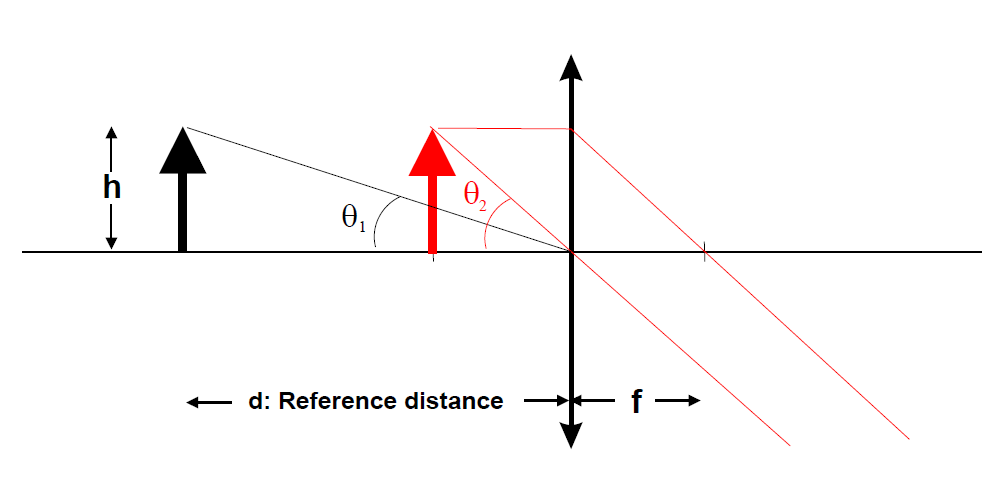
\includegraphics[width=120mm]{images/Angular_magnification.png}
\caption{Angular magnification at short distances\label{angular}}
\end{figure}

Though using lenses is a way of corrected for testing at short distances, a few problems arise from this. Figure \ref{angular} shows the problem of angular magnification. 

The magnification is a problem is visual acuity testing because if the optotypes on the eye chart are enlarged then an error will show up in the results.

\newpage
\begin{figure}[h]
\centering
\begin{tabular}{| l | l | l | l |}
    \hline
    Distance to chart (m) & Addition (D) & Magnification (Rel.) & Error (logMar) \\ \hline
    4                     & 0.25         & 1.5                  & 0.17           \\ \hline
    2                     & 0.5          & 3.5                  & 0.48           \\ \hline
    1                     & 1            & 6.0                  & 0.78           \\ 
    \hline
    \end{tabular}
    \caption{Magnification due to addition for closer distance\label{magtable}}
\end{figure}

There is need to have a standard to follow on how much addition or subtraction needed for a specific distance. Figure \ref{magtable} shows what values to use when testing visual acuity at shorter distances than six meters. \cite{PGSoderberg}

\section{Chart Design}
The visual acuity charts used in this project are based on the ETDRS (fig. \ref{fig:etdrs_chart1}, page \pageref{fig:etdrs_chart1}) \cite{Ferris} and the Axanivis (fig. \ref{fig:axanivis}) \cite{PGSoderbergOral} charts developed by P.G. Söderberg at Uppsala University Hospital. 

%\begin{figure}[ht!]
%\centering
%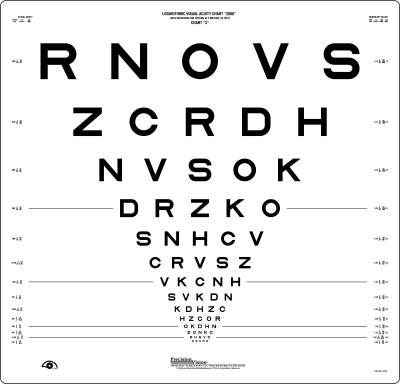
\includegraphics[width=100mm]{images/etdrs_chart.jpg}
%\caption{Example of a ETDRS chart used with permission from Precision Vision \\ (Source: http://precision-vision.com/)\label{fig:etdrs_chart}}
%\end{figure} 

\subsection{Optotypes} \label{Optotypes}
An optotype is a symbol that is used on a visual acuity chart. The optotypes are all of the same width and height and placed on a five by five grid. The most common type of symbol to use are letters from the Latin alphabet but can be different depending on the patient's needs\cite{Colenbrander}.

\textit{Sloan letters} are defined to be the ten optotypes \textit{C, D, H, K, N, O, R, S, V and Z}. They have been chosen because they are easily differentiated from each other \cite{Ferris} and are used by most visual acuity charts\cite{Colenbrander}.

\textit{Landholt C} is a sloan \textit{C} that is rotated by 0, 90, 180 or 270 degrees and is usually used in a scientific environment. The Landholt C is used as reference when deciding the how difficult it is to read a specific optotype\cite{Colenbrander}.

\textit{Tumbling E} is like the Landholt C, but with the optotype \textit{E} instead of \textit{C}. This optotype can be used instead of the Sloan collection of optotypes if the patient doesn't know how to read. The patient can instead show or tell the optician in what direction the \textit{E} is rotated\cite{Colenbrander}.

\textit{HVOT} are the letters \textit{H},\textit{V},\textit{O} and \textit{T}. These letters are chosen because they look the same if they are mirrored on the horizontal axis.

\textit{LEA} are four symbols that look like a house, circle, box and apple. These symbols similar to HVOT since they look the same if you mirror them on the horizontal axis.

\begin{figure}[ht!]
\centering
\begin{subfigure}{.3\textwidth}
  \centering
  
\includegraphics[width=.4\linewidth]{images/landholt_c_optotype.png}
  \caption{Landholt C}
  \label{fig:landholt_c}
\end{subfigure}%
\begin{subfigure}{.3\textwidth}
  \centering
  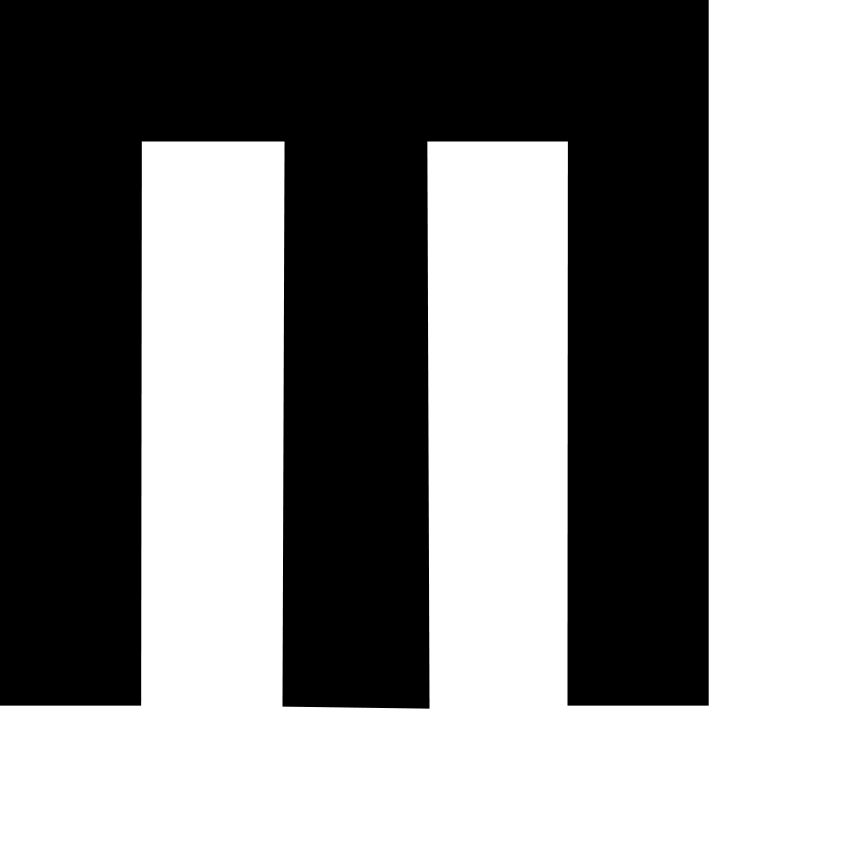
\includegraphics[width=.4\linewidth]{images/tumbling_e_optotype.png}
  \caption{Tumbling E}
  \label{fig:tumbling_e}
\end{subfigure}
\begin{subfigure}{.3\textwidth}
  \centering
  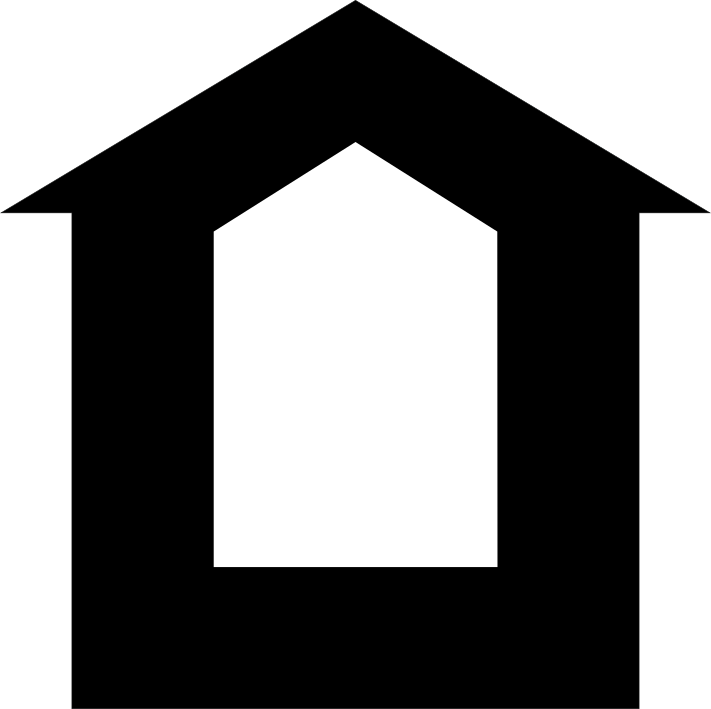
\includegraphics[width=.4\linewidth]{images/lea_optotype.png}
  \caption{LEA}
  \label{fig:lea}
\end{subfigure}
\caption{Some example optotypes}
\label{fig:optotypes_example}
\end{figure}

\pagebreak
\subsection{ETDRS Chart}
The ETDRS chart consists of fourteen rows with five optotypes on each row. The size of each optotype is measured in LogMAR which is the base 10 logarithm of the angle of one fifth of an optotype (eq. \ref{eq:logmar} and fig. \ref{fig:logmar_calculation}) \cite{Bailey}. The angle unit is measured in arcminutes, where one arcminute is $\dfrac{1}{60}$ degrees or $\dfrac{\pi}{10800}$ radians. If the angle v in figure \ref{fig:logmar_calculation} is equal to 8 arcminutes, then the size of the letter would be $log_{10}(8) \approx 0.903\ LogMAR$.

%\begin{figure}[h]
%\centering
%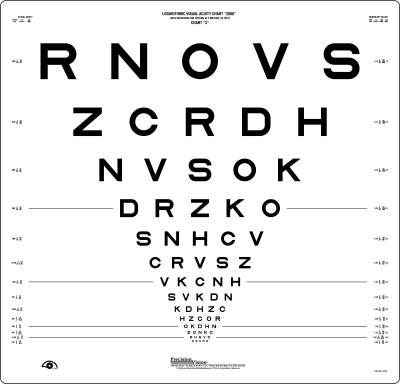
\includegraphics[width=100mm]{images/etdrs_chart.jpg}
%\caption{Example of a ETDRS chart \\ (Source: http://precision-vision.com/)%\label{fig:etdrs_chart}}
%\end{figure} 

\begin{equation}
	\begin{split}
  		LogMAR & = log_{10}(angle)
  	\end{split}
  	\label{eq:logmar}
\end{equation}

\begin{figure}[ht!]
\centering
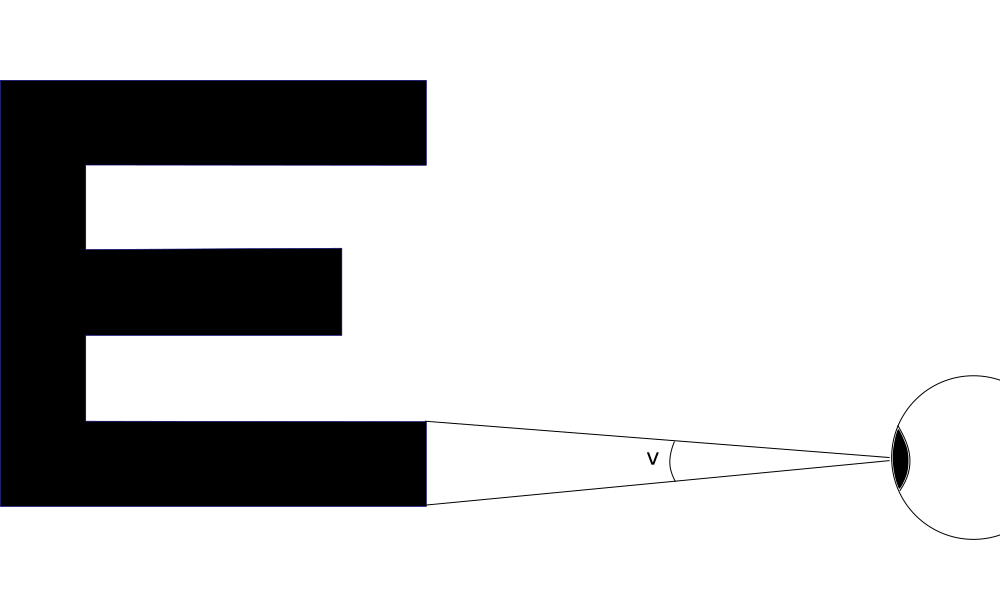
\includegraphics[width=110mm]{images/logmar_calculation.png}
\caption{The angle v is used to calculate the size in LogMAR of the optotype.(Source: Christian Johansson)\label{fig:logmar_calculation}}
\end{figure} 

The optotypes on the top row of the chart is of the size 1.0 LogMAR and then each row below is decremented by 0.1 LogMAR to the last row which is -0.3 LogMAR. This means that each optotype is approximately 1.2589 the height of the optotypes on the row below (fig. \ref{fig:chart_size_plot}) \cite{Ferris}. The spacing between each optotype is equal to the width of an optotype from the same row and the spacing between each row is equal to the height of an optotype on the lower row (fig. \ref{fig:etdrs_chart_sizes}).

\begin{figure}[ht!]
\centering
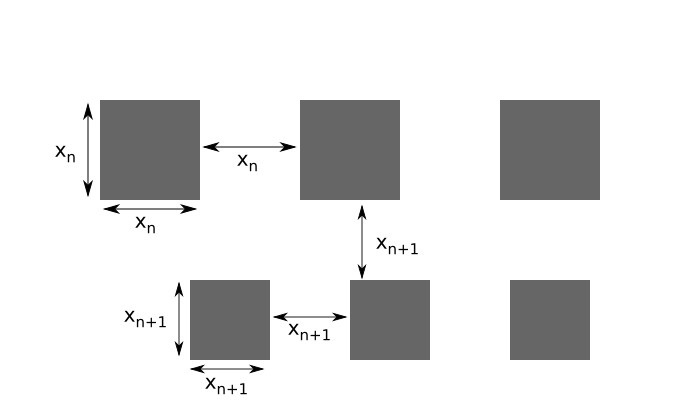
\includegraphics[width=110mm]{images/etdrs_chart_sizes.png}
\caption{The sizes and positions of the first three optotypes of row $n$ and $n+1$ where $x_n \approx 1.2589 x_{n+1}$. \label{fig:etdrs_chart_sizes}}
%\caption{The gray squares represents optotypes that on the upper row has a width and height of $x_n$ and on the lower row $x_{n+1}$.  \label{fig:etdrs_chart_sizes}}
\end{figure} 

\begin{figure}[ht!]
\begin{tikzpicture}
    \begin{axis}[
      xmin=1,xmax=14,
      ymin=0,ymax=180,
      xlabel={row},
      xlabel near ticks,
      ylabel={pixels},
      ylabel near ticks
    ]
      \addplot[color=blue, mark=*, only marks] plot coordinates{(1,162)(2,128)(3,102)(4,81)(5,64)(6,51)(7,41)(8,32)(9,26)(10,20)(11,16)(12,13)(13,10)(14,8)};
    \end{axis}
\end{tikzpicture}
\caption{The height of optotype from 2 meters on a 15.6" screen with a resolution of 1920x1080 pixels. (Source: Christian Johansson)\label{fig:chart_size_plot}}
\end{figure}

%\newpage
\subsection{Axanivis Charts}
The Axanivis charts are an extension to the ETDRS chart that modifies the original chart and adds two new chart layouts and digitalizes them so they can be displayed on a screen. Since the original ETDRS chart is made for a physical chart, it doesn't have an aspect ratio \cite{Ferris} that is close to a common monitor. To solve this, the original chart is split into an upper (fig. \ref{fig:etdrs_upper}) and a lower chart (fig. \ref{fig:etdrs_lower}). The upper chart consists of the five first rows and the lower chart consists of the the remaining nine.

\begin{figure}[ht!]
\centering
\begin{subfigure}{.8\textwidth}
  \centering
  %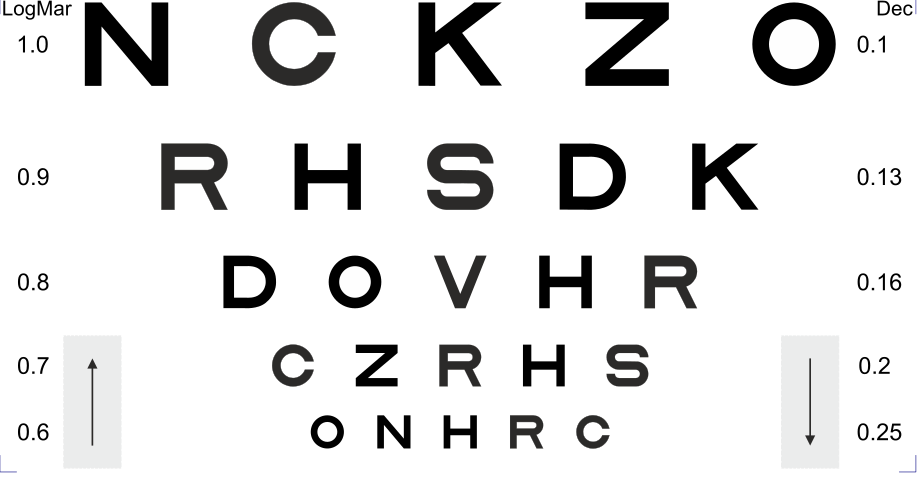
\includegraphics[width=.5\linewidth]{images/etdrs_top.png}
  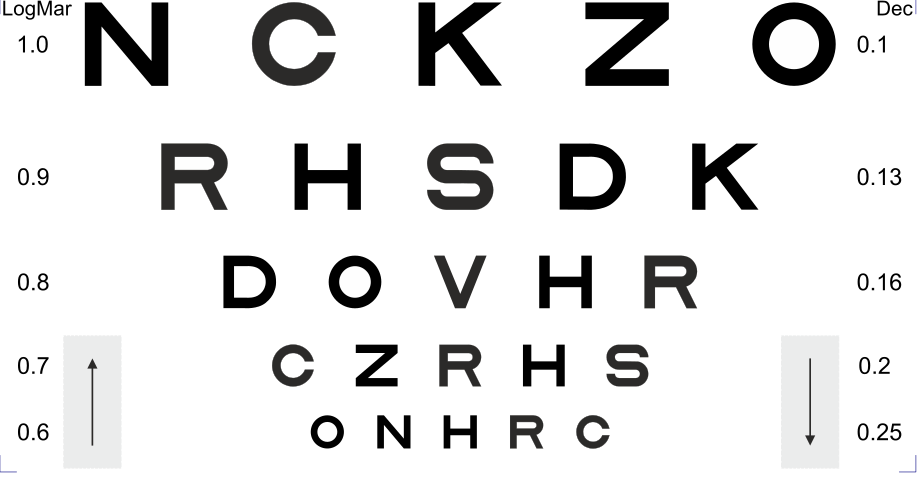
\includegraphics[width=100mm]{images/etdrs_top.png}
  \caption{Upper Chart}
  \label{fig:etdrs_upper}
\end{subfigure}%

\begin{subfigure}{.8\textwidth}
  \centering
  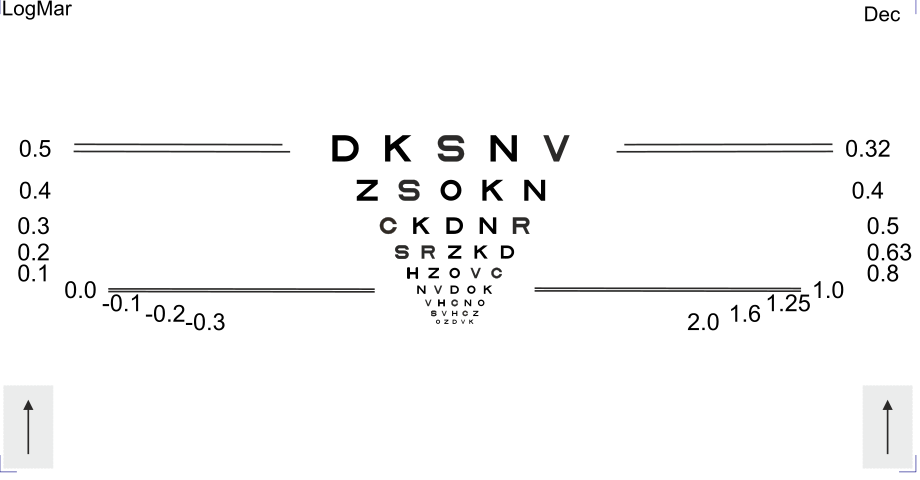
\includegraphics[width=100mm]{images/etdrs_bottom.png}
  \caption{Lower Chart}
  \label{fig:etdrs_lower}
\end{subfigure}
\caption{The upper and lower ETDRS charts (Source: P.G. Söderberg)}
\label{fig:etdrs_upper_lower}
\end{figure}

The two new chart layouts used is constructed using the same principles, like height and spacing of optotypes, as the original ETDRS chart. But instead of having 14 rows of 5 optotypes each, the first new layout takes a single column of the ETDRS chart and rotates it 90 degrees (fig. \ref{fig:etdrs_one_line}) so it's all on one line. This makes it wider than it's high which suits a monitor better. This also allows the patient to read from left to right, which is the common way to read in Europe and America. This makes it easier and feel more natural to read for a patient used to read in English or any other European language \cite{PGSoderbergOral}. Since the patient only have to read one letter of each size, this layout gives a quicker but more inaccurate result. This is useful to get a quick estimate on the visual acuity of the patient.

\begin{figure}[ht!]
\centering
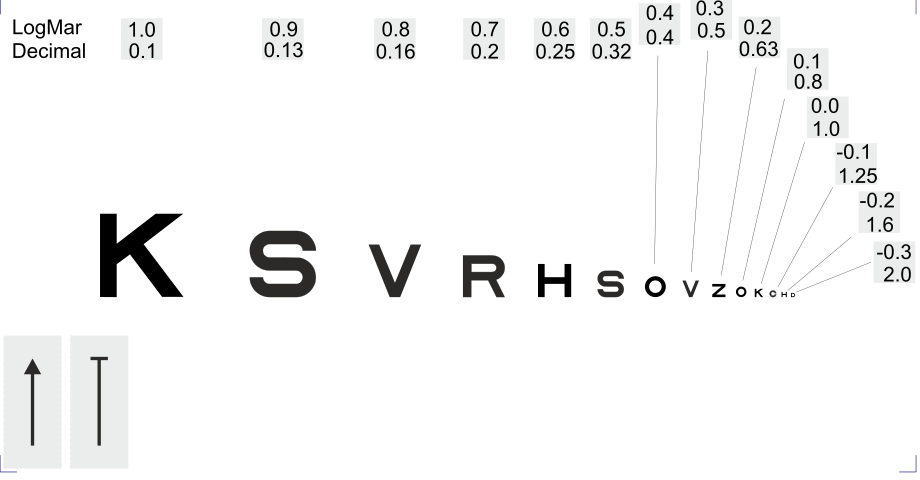
\includegraphics[width=100mm]{images/etdrs_one_line.png}
\caption{The one line chart (Source: P.G. Söderberg)}
\label{fig:etdrs_one_line}
\end{figure}

\pagebreak
Once an estimated visual acuity has been achieved from the one line chart, the user can select an optotype and show the second new layout, which will only display one optotype at a time (fig. \ref{fig:etdrs_single}). This layout allows the patient to easily focus on a single optotype at a time. The user can then page between the different optotype sizes in order to determine the visual acuity.

\begin{figure}[ht!  ]
\centering
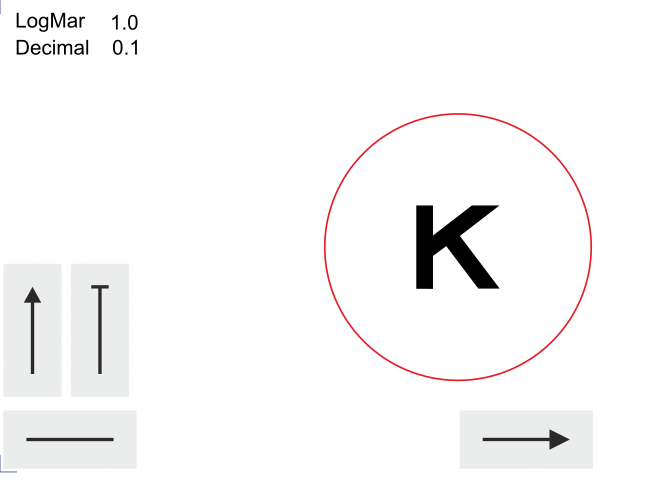
\includegraphics[width=90mm]{images/etdrs_single.png}
\caption{The single optotype chart where the red circle indicates the area the patient should focus on.}
\label{fig:etdrs_single}
\end{figure}

\chapter{ Implementation}
\section{Methods}
\subsection{System structure}
The system is divided into three major parts, an Android application, a server and networking. The Android application and server is modeled after the MVC (Model-View-Controller) pattern, where the model is the logic, such as calculating the sizes of the optotypes and randomizing the order which they appear, and the view is the GUI (Graphical User Interface). The controller part is the part on the Android application that listens for button clicks and gestures. Usually the networking would fall under controller in the MVC pattern but was, in this system, chosen to be a separate larger structure. The reason the network part is separated from the controller is because it is large part of the system and it separates the project into three parts. This allows each project member to focus on a single part. Figure \ref{system_structure} shows how the different parts are connected.

\begin{figure}[ht!]
\centering
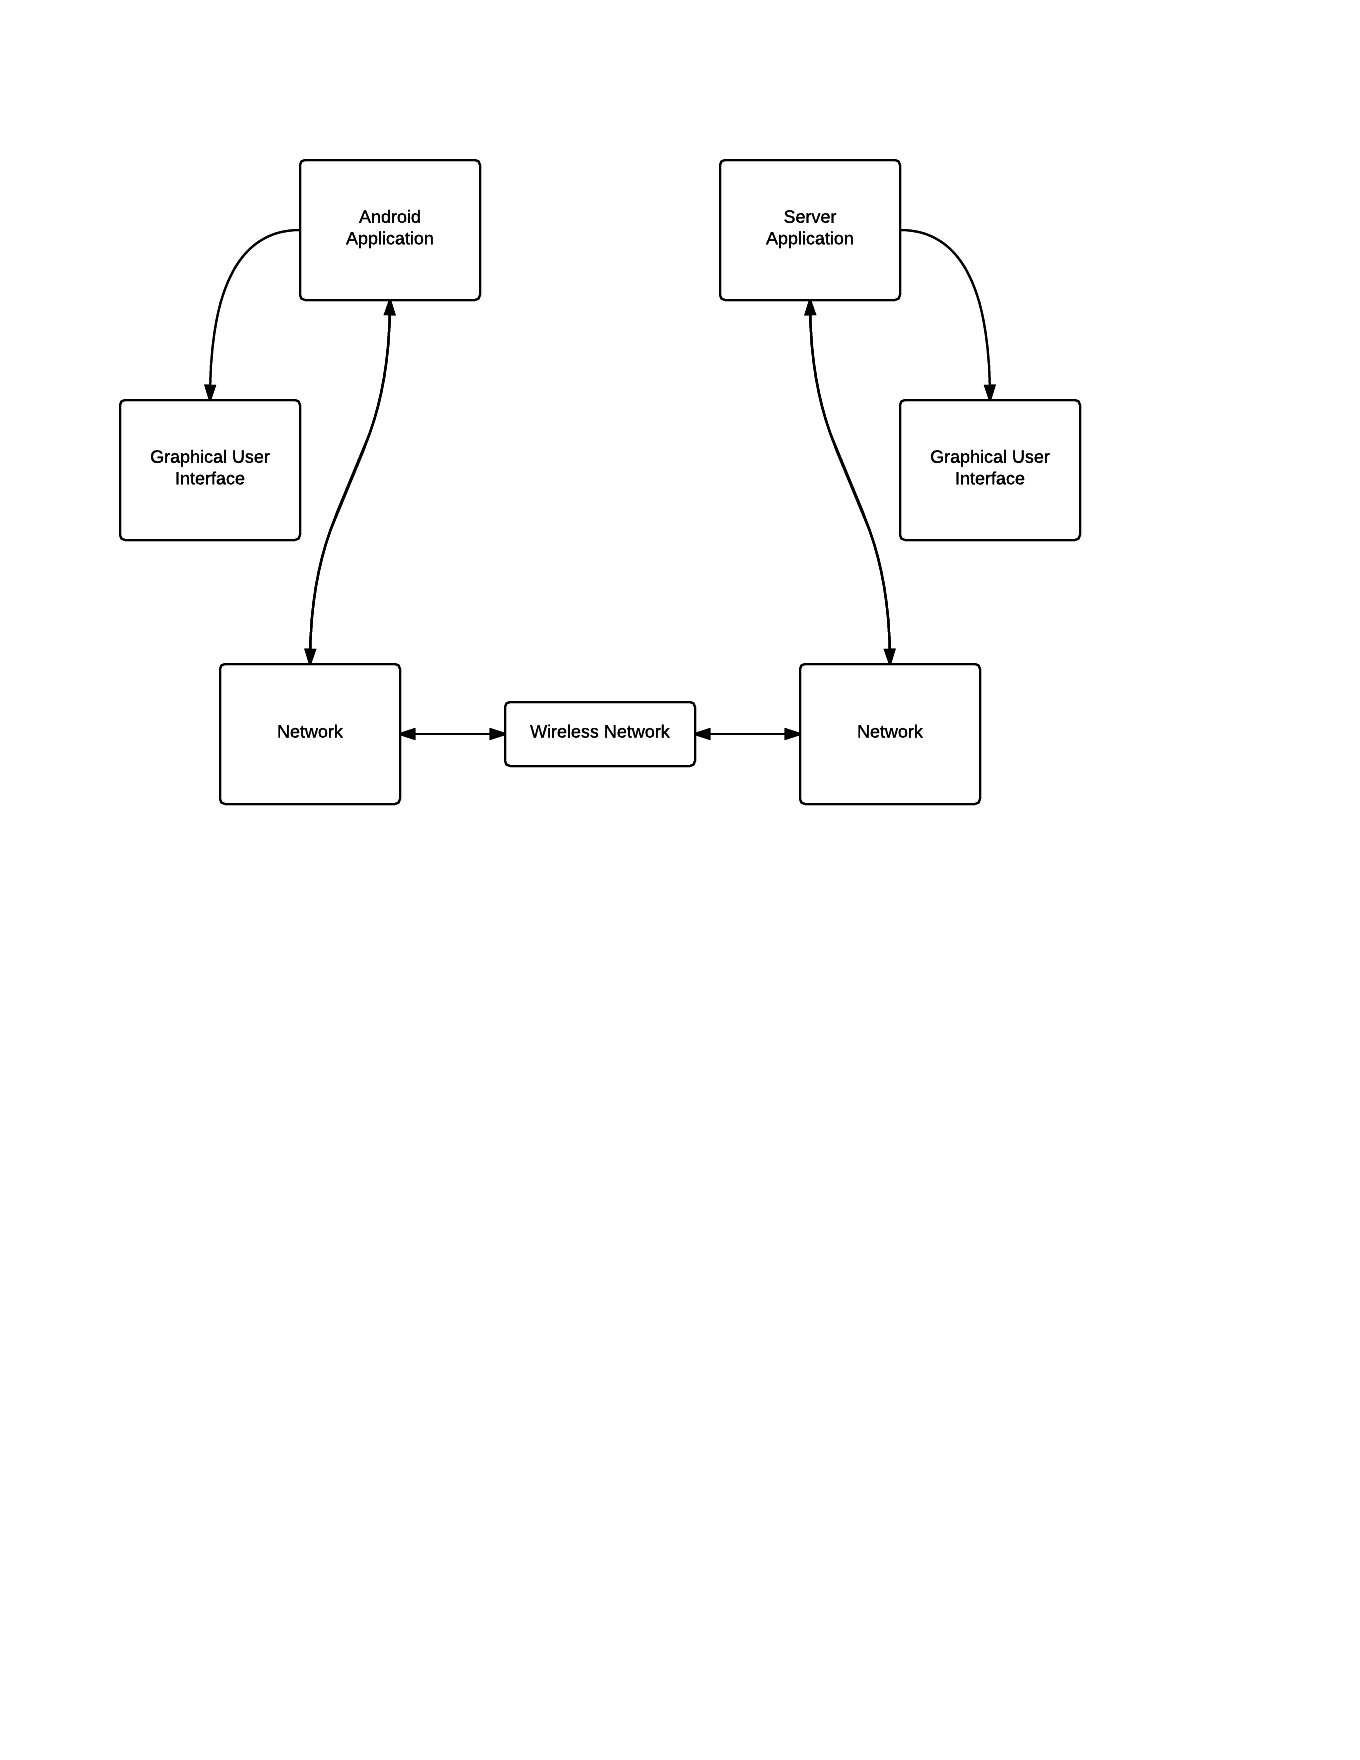
\includegraphics[width=90mm]{images/system_structure.png}
\caption{Overview of the system structure\label{system_structure}}
\end{figure}

\subsection{Android application}
The Android application is written in Java, which is the official language for Android. The static parts of the GUI, which will never change unless application updates are released, are written in XML using Googles defined syntax \cite{android_gui}. This is similar to how HTML is written and is supported by Android natively.

The visual acuity charts on the Android device have its opotypes positions and sizes calculated at runtime before before they are displayed. If the charts would have been written in an XML file, it would have required that each optotype had its own XML element with a manually inserted size and position. This would result in very large and hard to read XML files and would require manual updating of each element if the sizes or positions should ever change. The charts are all drawn at the same time and on top of each other, but makes all but the chosen chart invisible. This makes it seem like only one chart is calculated at a time and avoids recalculating when switching back and fort between charts.

The optotypes provided to us by P.G. Söderberg was created in the SVG (Scalable Vector Graphics) format which is a format that Android does not natively support. One possibility would be to convert the files to scalable fonts, but instead a third party library called AndroidSVG \cite{AndroidSVG} was used. This allowed us to avoid manipulating the optotype files and was considered to be the simplest solution.

% As Android does not natively have support for vector graphics and the chart optotype images are vector images the AndroidSVG library is used to display them \cite{AndroidSVG}.

The size of the optotypes is calculated using equation \ref{eq:optotype_size}, where $d$ is the distance in centimeters, $v$ is the angle in radians and $h$ is the height of the optotype in centimeters.

\begin{equation}
	\begin{split}
  		2d\ tan(\frac{v}{2}) & = h
  	\end{split}
  	\label{eq:optotype_size}
\end{equation}

The settings, such as the distance from the screen the patient is watching or the order which the optotypes appear, associated to each chart are also generated at runtime. If this were not the case, every different version of the chart would need its own XML file, as each version contains a different number of predefined charts.

In order to control the application, \textit{listeners} were created to listen to button clicks and gestures when the user attempts to interact with the application. The listeners are Java classes that contains methods which are connected to an interactive object on the screen, such as a button. Whenever a user interacts with an interactive object on the screen, the corresponding method in the listener is called. This method, in turn, calls other methods in order to perform the user requested action. The use of listeners separates the user input from the logic and creates a simple way of changing the functionality of an interactive object by letting the object call another listener method instead.

The design of the application follows the Android design principles by using Androids built in navigation drawer (fig. \ref{fig:example_nav_drawer}) and the built in views i.e. buttons, radio buttons, lists etc. \cite{android_design}.

\begin{figure}[ht!]
\centering
\begin{subfigure}{.5\textwidth}
  \centering
  %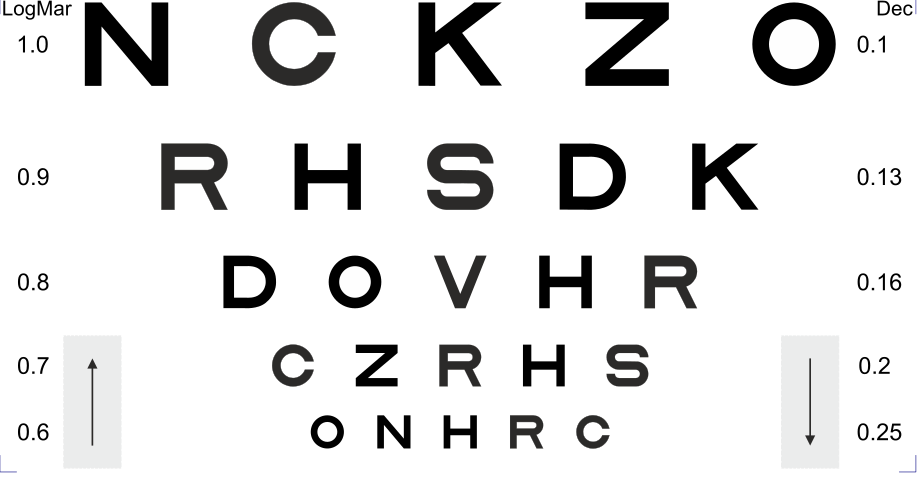
\includegraphics[width=.5\linewidth]{images/etdrs_top.png}
  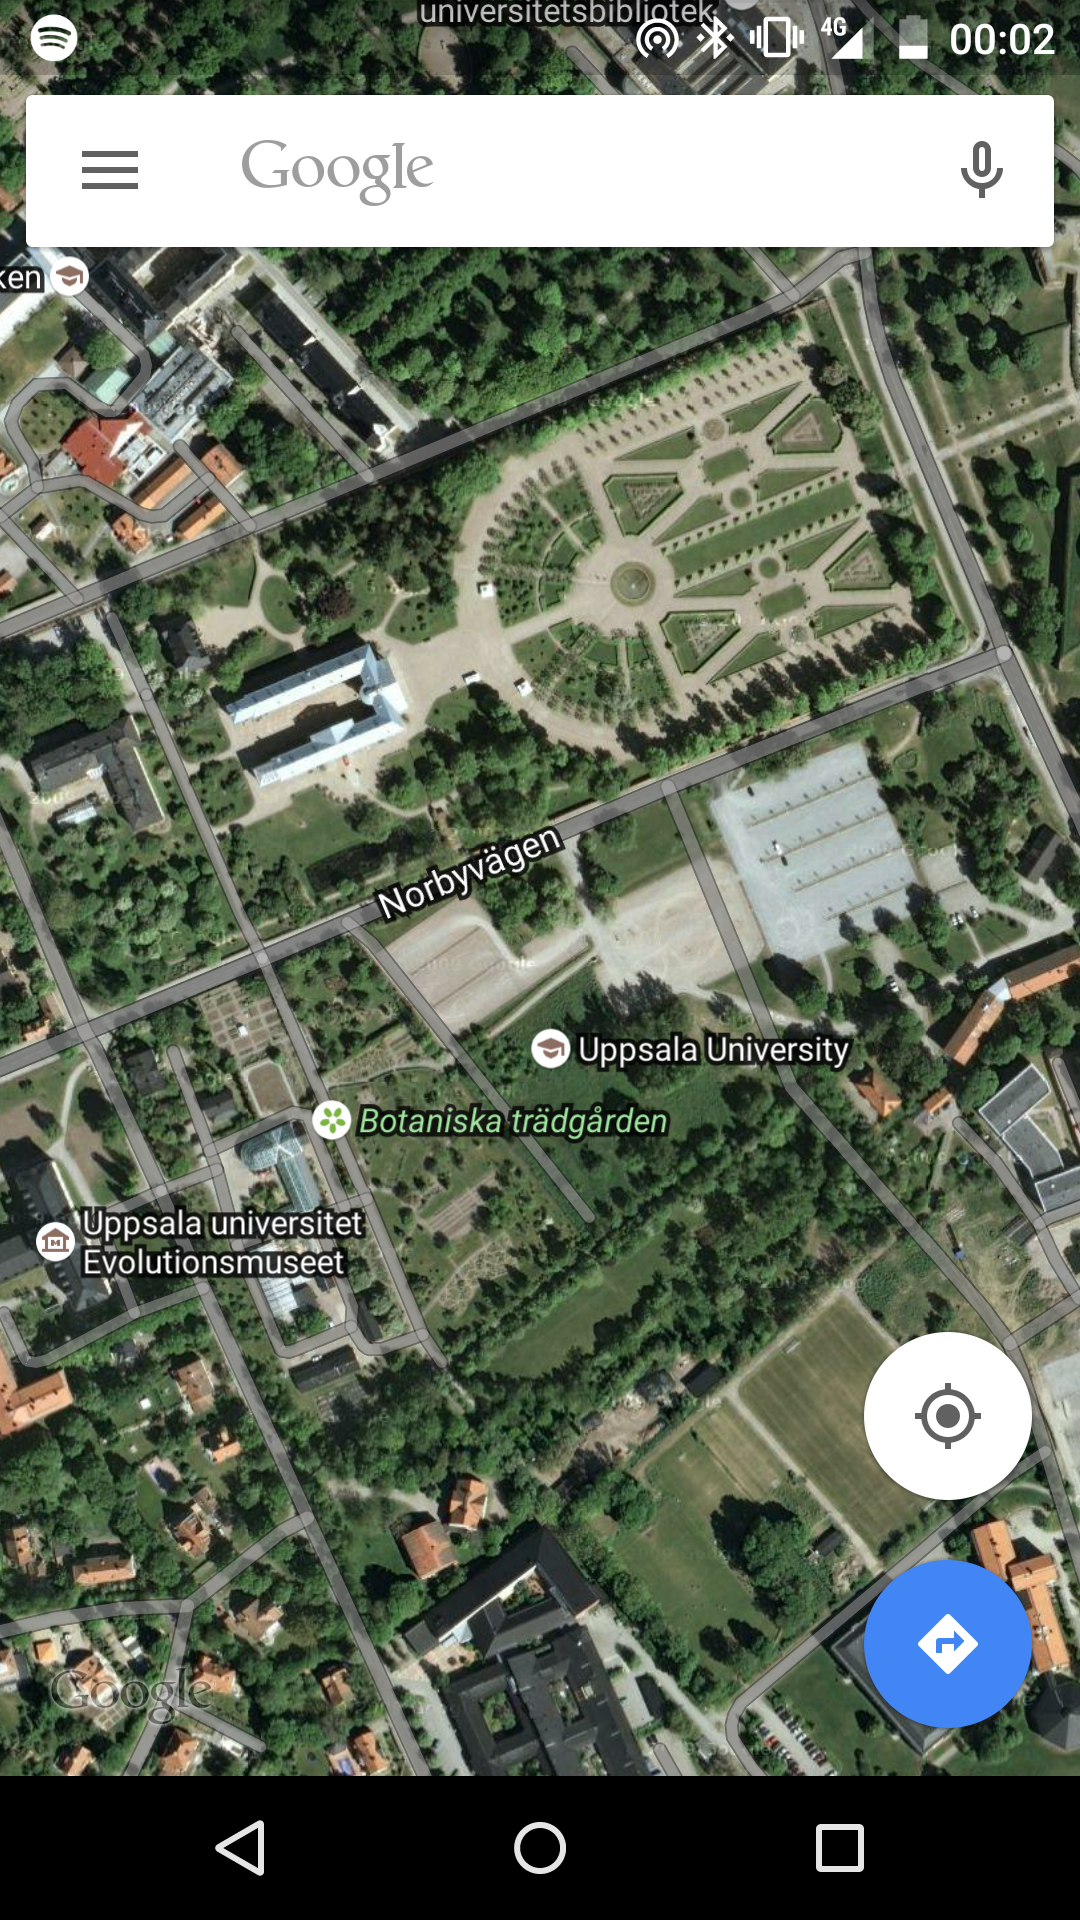
\includegraphics[width=50mm]{images/no_nav_drawer.png}
  \caption{A closed navigation drawer which can be opened by clicking on the three lines on the top left of the screen or by swiping from the left edge of the screen to the right.}
\end{subfigure}%
\begin{subfigure}{.5\textwidth}
  \centering
  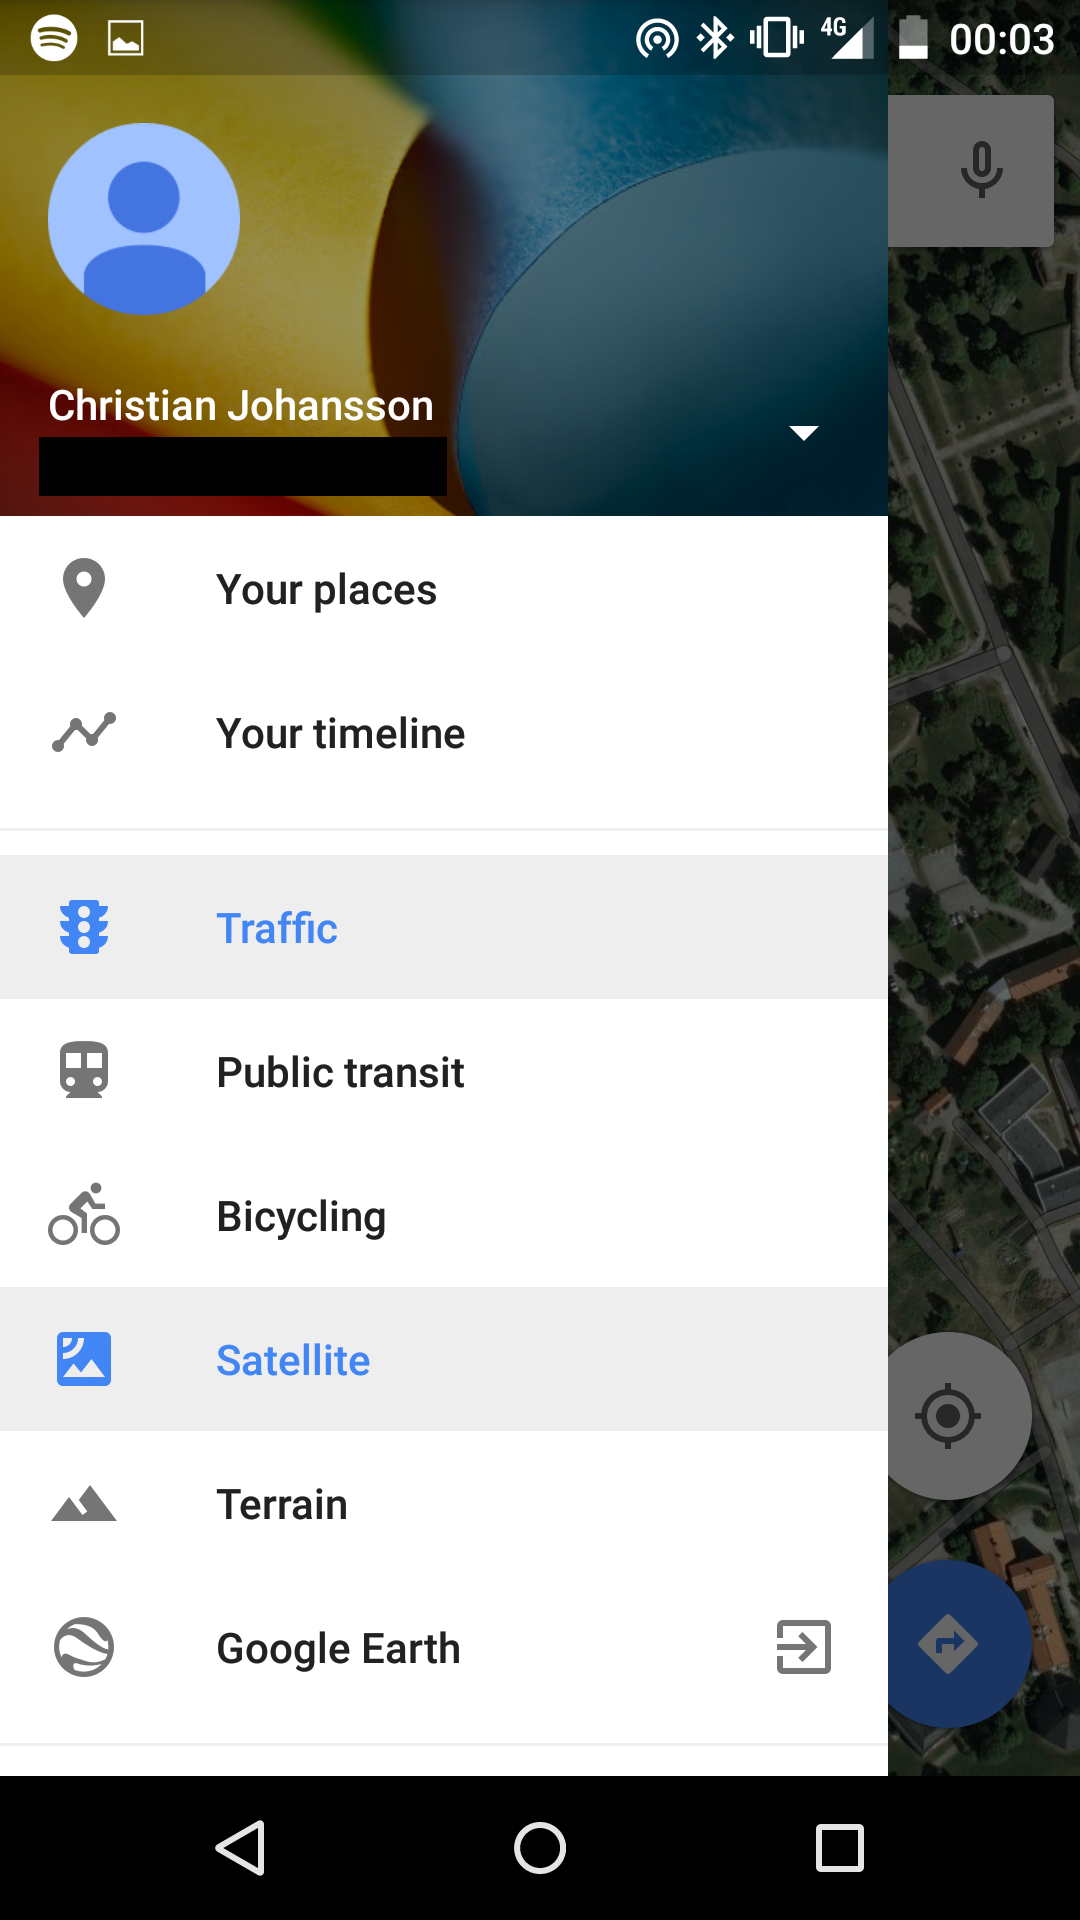
\includegraphics[width=50mm]{images/nav_drawer.png}
  \caption{An open navigation drawer which can be closed by pressing the back button or by swiping from the right to the left.}
\end{subfigure}
\caption{An example on how Google Maps navigation drawer looks like. (Source: Christian Johansson)}
\label{fig:example_nav_drawer}
\end{figure}

\subsection{Server application}
The server application is written in Java and uses the built-in \textit{Swing} library for drawing the GUI and the images. Swing is a very flexible and easy-to-use library with a lot of great tools for creating a good looking GUI. In our case
we won't be needing a very advanced GUI since the main purpose of the server is to render a fullscreen image at all times. This greatly simplifies the implementation of the GUI. Other than the rendering of images, the GUI will consist of a small network controller where the user can specify a number of settings. These settings will be needed to configure for example what name the server will have on the network. It's also necessary to have settings for the location of the server.

The rendering of images, specifically SVG vector graphic images, will be handled by an \textit{~Apache} library called \textit{Batik}. It is well supported and extensive library for rendering a multitude of different file formats. The SVG files contain information about the optotypes used on the charts. Using procedural positioning of the SVG images, we can easily create a well structured image to render to the screen.

%The server will also handle the networking on its side, connecting to the Android tablet over a TCP connection. This will be done using a third-party library \textit{Kryonet}. \cite{kryonet} Kryonet is a library that wraps Java's own networking functionality and improves upon it. The library's strong-point is the way it implements serialization of Java objects. Using Kryonet we can without a lot of effort serialize objects, send the object over the network and then deserialize is, getting back the original object with all of its internal structure. 

Network communication will be handled using a submit-poll system. The networking part of the server will receive information from the network and submit it to a thread-safe queue. While this happens, the GUI polls the information from the queue and handles the information. This methods is necessary because of how Swing is constructed. Swing runs on a dispatch-thread basis, meaning only the dispatch-thread itself can change things in the GUI. Trying to change things in the GUI from another thread would cause a lot of problems. Now the GUI can try to poll whenever it has time, though tries to do this periodically.  

\subsection{Network}
The network communication between the client and the server consists of two parts. The first part is server detection and the second is server communication. All network communication are handled in threads separate from the main thread using Java's SwingWorker- and Androids AsyncTask class. Both classes allow us to perform network operations in the background, in a separate thread, and once the operations are complete the main thread of the program will automatically get the result.


\subsubsection{Server detection}
In order to detect all servers on the network, the Android application sends out a discovery request message, consisting of the string \\ \textit{AXANIVIS\_DISCOVER\_REQUEST}, 5 times with a 1 second interval using UDP (User Datagram Protocol) on the networks broadcast address using port 14141. The server, which constantly listen for broadcasts containing the correct message, will then respond to that message with the message \textit{AXANIVIS\_DISCOVER\_RESPONSE\textbackslash nServerName}, again using UDP. Once the Android application receives a response it adds the server to a list. The user can then choose to connect to one of the found servers or attempt the detection again if no servers were found.

Since UDP is a connectionless protocol, there is no guarantee that the server actually receives the message, the discovery request message is sent 5 times, which means the server have 5 chances to receive the message and respond to it. This means that the server will receive a discovery request 0 to 5 times and respond to it the same number of times. To avoid duplicate server entries in the list, a server is only added if it doesn't already exist in the list.

%In order to detect all servers on the network, the Android application sends out a UDP (User Datagram Protocol) broadcast message containing server discovery request. The application will then listen for incoming server responses. Once the application haven't received anything for three seconds from the last server response, it will stop listening and determine that all available servers have responded. The names and addresses of the servers will then be extracted from each response message and stored in a list so the user can choose which one to connect to.

%The servers themselves are constantly listening for broadcasts containing the server discovery request. Once a request is received, the server will send a response and then keep listening for more requests.

\subsubsection{Server communication}
The communication between the Android application and the connected server is handled using strings of characters divided to three lines using line separators. The first line consists of a check word, which is the same for every message. If this check word is wrong or doesn't exist, the server will ignore the message. The second line is the command to the server. This could be a command to set the current chart type or size to something else. The third line is the data required for the command. The data can be empty (null) or a string of characters. Depending on the command, the string of characters can be read as either a sequence of ASCII characters or a sequence of numbers. The messages defined for the server communications are commands to connect to the server, set the distance from the screen and set which chart to be displayed with which optotype. If a message with an incorrect command is sent to the server, the server will ignore that message. If the wrong data is sent together with a correct command, the server will keep functioning but its output is undefined.

The messages are sent using a TCP (Transmission Control Protocol) connection to the server on port 14142. This guarantees that the entire message will be correct and that it will be retrieved by the server as long as the server is connected to the network. If a connection is timed out, the sent command is ignored and the user have to reconnect to a server and resend the command.

%The communication between the client and server is handled using simple TCP (Transimission Control Protocol) messages. The TCP messages are used for sending and receiving commands and are structured as three lines of text (Example \ref{tcp_message}). The first line is a \textit{check} word and is the same for every \textit{command}. The second line is a \textit{command} word which tells the receiver what to do and the third line is the \textit{data} required for the \textit{command}. In many cases the simple \textit{command} is enough and the \textit{data} is left empty.

%\begin{center}
%\renewcommand{\lstlistingname}{Example}
%  \lstset{%
%    title=Example of TCP message,
%    basicstyle=\ttfamily\footnotesize\bfseries,
%    xleftmargin=.2\textwidth, xrightmargin=.2\textwidth
%  }
%\begin{lstlisting}[caption=TCP Message, label=tcp_message]
%CHECK_WORD
%LARGE_CHART
%NULL
%\end{lstlisting}
%\end{center}

\begin{figure}[h]
  \lstset{%
    basicstyle=\ttfamily\bfseries,
    xleftmargin=.4\textwidth, xrightmargin=.2\textwidth
  }
\begin{lstlisting}
AXANIVIS
DISTANCE
500
\end{lstlisting}
\caption{An example of how a network message that sets the distance from the screen to 500cm.
%A message with the check word \textit{AXANIVIS}, the command \mbox{\textit{DISTANCE}} and the data \textit{500}. This message would make the server to resize the currently active chart to be suitable for a user watching from 500 centimeters. 
\label{fig:example_message}}
\end{figure}

%\section{Boundaries (OLD!)} 
%%%%%%%%%%%%%%%%%%%%%%%%%Avgränsningar: vad ska INTE göras, även om man kanske kunde tro det?
%We are not tasked to develop a library to display .SVG files, and will be using a licensed one. We are also not tasked to populate the database with symbols and layouts, but instead provide a comprehensive API so that clients can create their own.
%
%%%%%%%%%%%%%%vad ska bara göras om tid/resurser/omständigheter räcker till?
%
%There are however several extensions to the system that can be considered if we have time to spare. We can extend the system to support more types of charts, such as charts for testing colour blindness and stereoscopic vision, which also rely heavily on rooms with appropriate lighting.
%
%While it deviates further from the main part of the project, we were asked by our employer to consider implementing the ability to control devices such as lights around the room from inside the app. This could probably be done, and we will look into it if time allows.
%
%\section{Demands (OLD!)} %%%%%%%%%%%%%%%%%%%%%%%%Krav: vilka krav ställer ni/andra på ert resultat? hur snabbt? hur många användare? hur strömsnålt? eller vad som är relevant
%There are a few core demands that our product needs to meet. First and foremost, it needs to work, and do what the current testing system can already do. Second, it needs to be easy to use and have an intuitive interface. Third, it should be very energy efficient, since forcing the user to recharge the tablet often reduces productivity. 
%
%\section{Evaluation (OLD!)} %%%%%%%%%%%%%%%%%%%%%%%%Utvärdering: hur ska ni utvärdera ert arbete/system, hur vet ni om/hur bra ni lyckats?
%The easiest way to see if our product satisfies these demands is putting it into the hands of the opticians at the university hospital and letting them test it, recording bug reports or comments. Testing will also let us determine if the system is as energy efficient as we intended.

\chapter{ Results}
\section{System functionality} 
%The system fulfills all specified requirements and allow the user to quickly set up a chart on the monitor. No system crashes have occurred during testing, and no bugs that causes the system to not work properly have been encountered. With a stable WiFi connection, the system runs smoothly without any lag and the server detection finds a server in under a second. 
The resulting system ended up in three parts, an Android part, a server part and a network part, as shown in the system structure (fig. \ref{system_structure}). Every action on the Android device related to a chart is connected to the network part. Once an action has been chosen, the network part is called and it creates a message with the correct command and data and then sends this message to the server. Once the server receives this message, the server will perform the requested actions.

\subsection{Android application}
The Android application uses Android's standard GUI elements. To navigate between the connection settings and different type of charts, Android's built in navigation drawer is used (fig. \ref{fig:app_nav_drawer}). In order to reach the connection settings, the user must click the name of the connected server and in the case that no server is connected, it will, instead of the name of a server, say \textit{Click to connect}.

\begin{figure}[ht!]
\centering
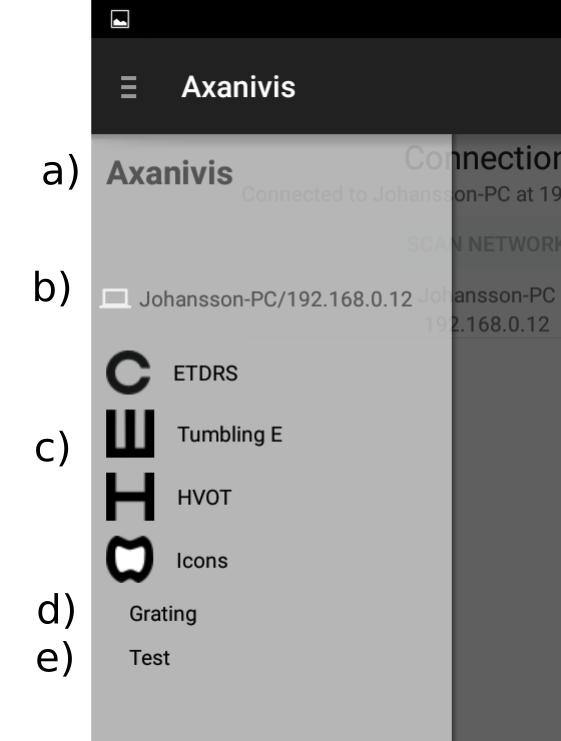
\includegraphics[width=56mm]{images/appgui/nav_drawer.png}
\caption{The Android application navigation drawer used for navigating the application. a) Name of the application b) The currently connected server c) Available optotypes d) Grating, not yet implemented e) Test, used for testing new functions}
\label{fig:app_nav_drawer}
\end{figure}

Once the connection settings page have been reached, the user will be shown the connection status and a \textit{scan network} button (fig. \ref{fig:scan1}) which can be used to scan the network for servers. Once the button is pressed, the button will be disabled and found servers will appear in a list below (fig. \ref{fig:scan2}). When the desired server has been found, the user can click on it to connect to it and once the entire scan is complete, the \textit{scan network} button will be enabled again.

\begin{figure}[ht!]
\centering
\begin{subfigure}{.5\textwidth}
  \centering
  %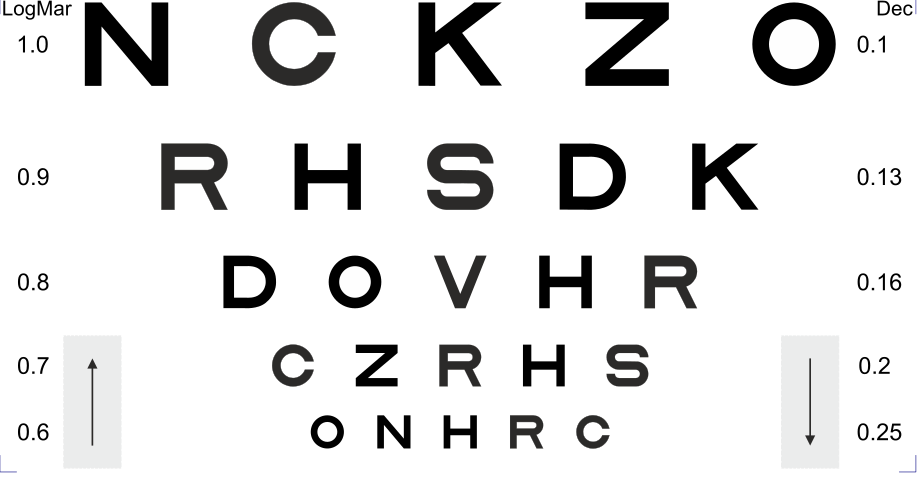
\includegraphics[width=.5\linewidth]{images/etdrs_top.png}
  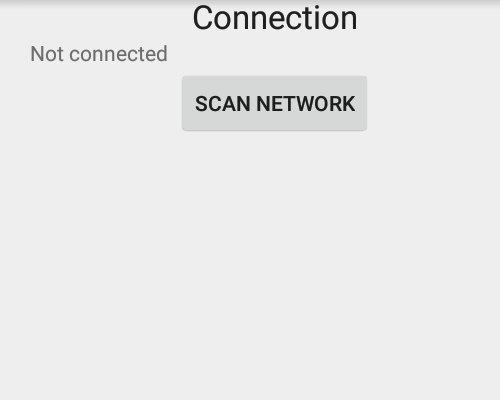
\includegraphics[width=50mm]{images/appgui/scan1.png}
  \caption{No connection}
  \label{fig:scan1}
\end{subfigure}%
\begin{subfigure}{.5\textwidth}
  \centering
  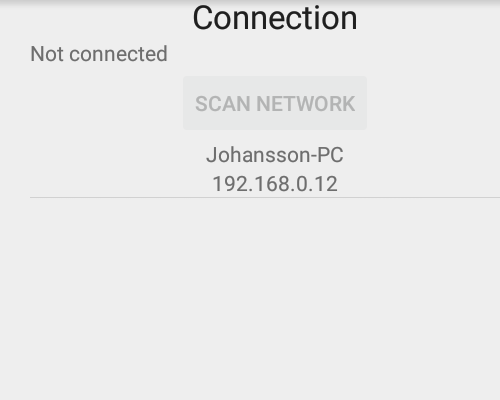
\includegraphics[width=50mm]{images/appgui/scan2.png}
  \caption{Scan button pressed}
  \label{fig:scan2}
\end{subfigure}
\begin{subfigure}{.5\textwidth}
  \centering
  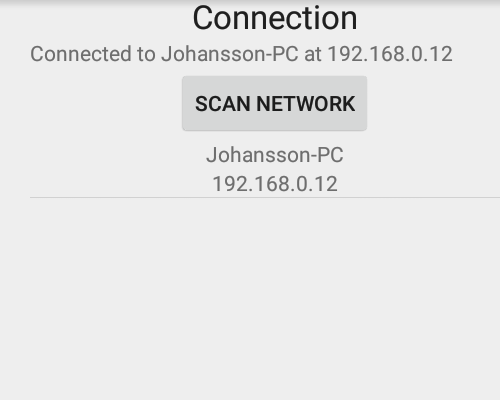
\includegraphics[width=50mm]{images/appgui/scan3.png}
  \caption{Connected to server}
  \label{fig:scan3}
\end{subfigure}
\caption{Server connection steps}
\label{fig:scan}
\end{figure}

Once the application has connected to a server, the user can navigate to the chart that should be viewed on the screen. This is done by opening the navigation drawer, either by swiping from the left edge of the screen to the right, or by pressing the navigation drawer icon in the top left corner. When the navigation drawer is open, the user can choose between the \textit{ETDRS} (Sloan letters), \textit{Tumbling E}, \textit{HVOT} or \textit{Icons} (LEA) to display that chart (fig. \ref{fig:etdrs_large}). 

\begin{figure}[ht!]
\centering
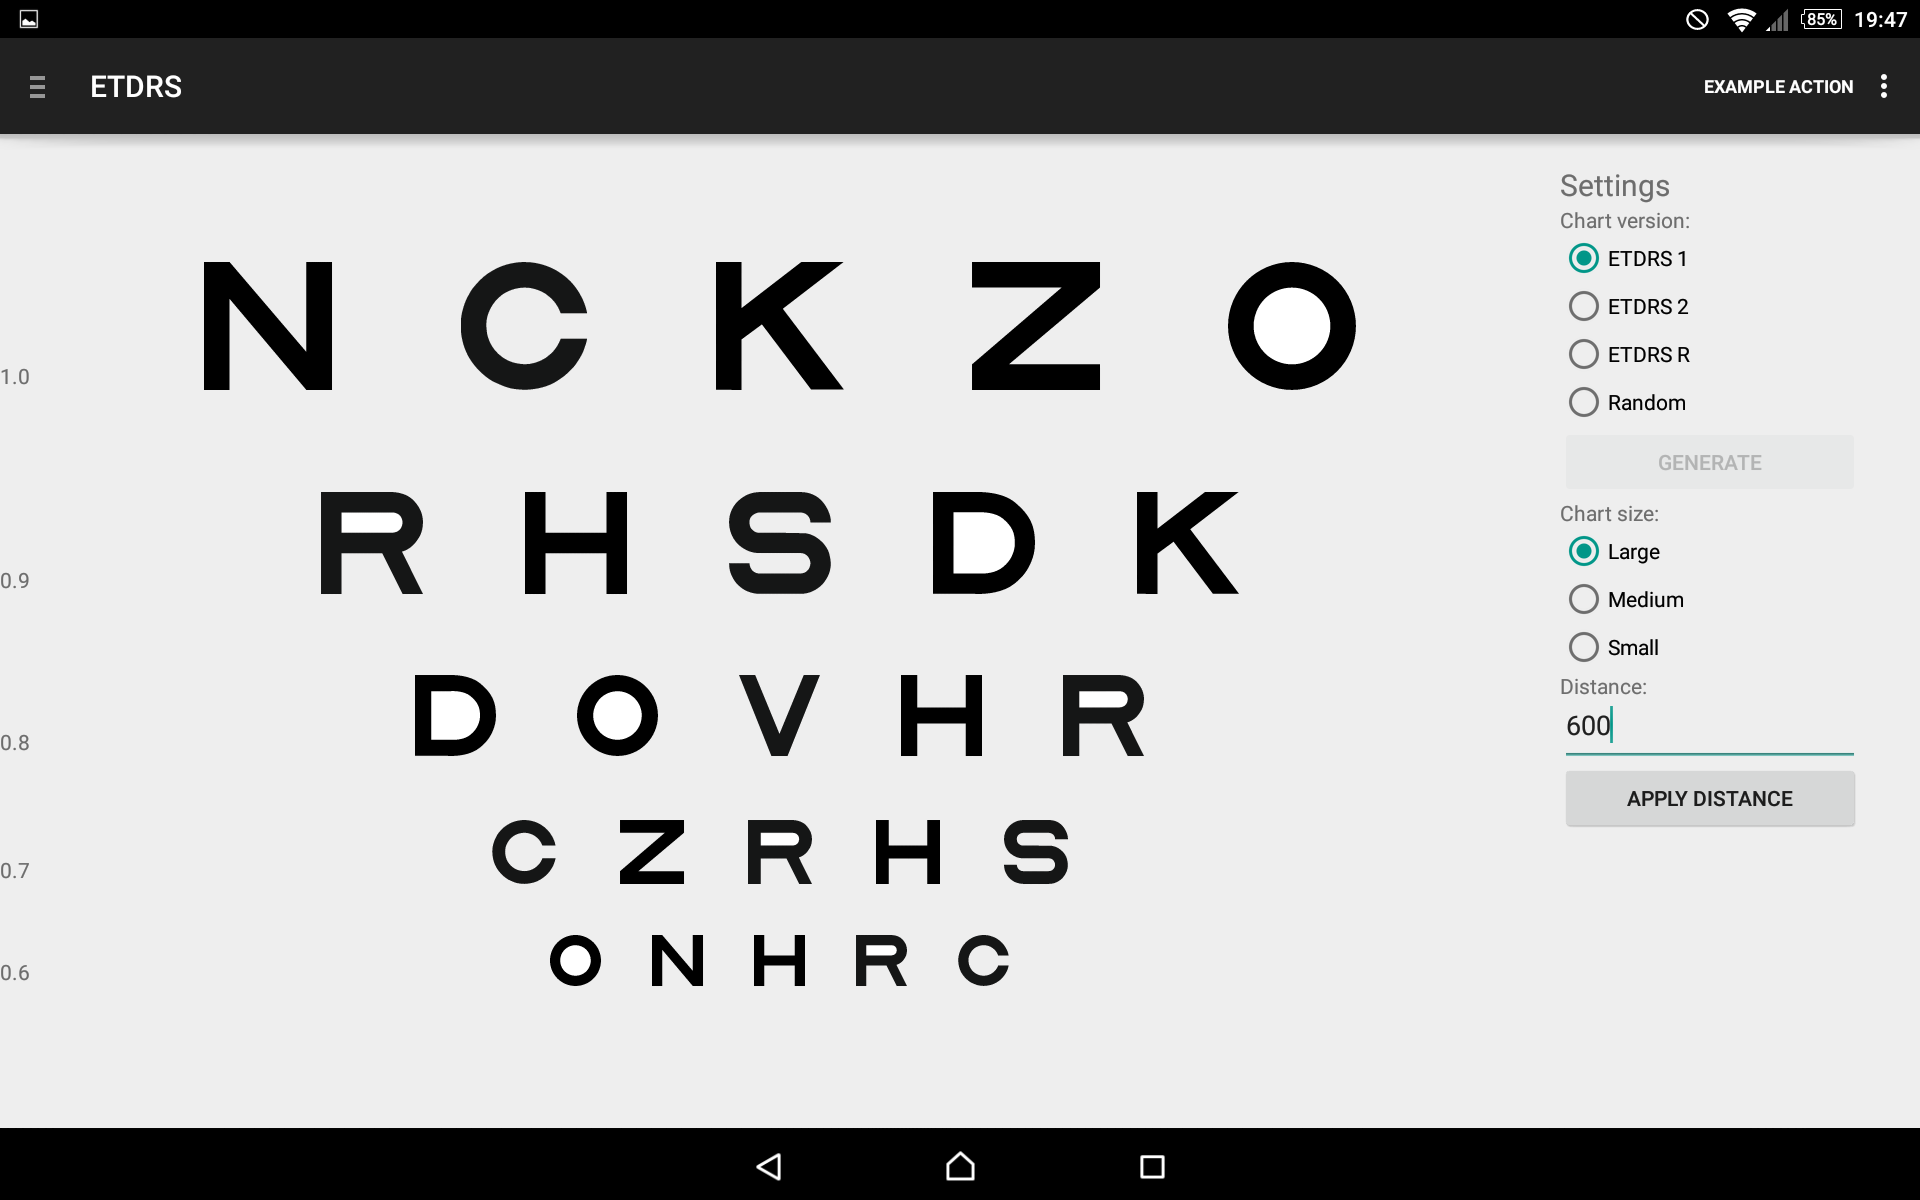
\includegraphics[width=120mm]{images/appgui/etdrs_large.png}
\caption{The upper large ETDRS 1 chart displayed with each rows LogMAR values to the far left.}
\label{fig:etdrs_large}
\end{figure}

The user can now choose which chart version, size and distance to use. The chart version decides which optotype to use at which position. The ETDRS chart has 3 pre-made versions\cite{Ferris} and the rest of the charts have 1. There is also an option to use a randomly generated version which is generated when the application starts. If the random version is selected, the generate button is enabled. The random version is generated with no restrictions and should be used with caution.

The user can also choose which chart size, \textit{Large}, \textit{Medium} or \textit{Small}, to use. The large chart is the same chart as the \textit{upper} and \textit{lower ETDRS} charts (fig. \ref{fig:etdrs_large}), the medium chart is the same as the \textit{one line chart} (fig. \ref{fig:icons_medium}) and the small chart is the same as the \textit{single optotype chart} (fig. \ref{fig:tumbling_e_small}). The reason the names in application differs from the names in the report is the result of an early design choice which will most likely change in the future. To navigate between the upper and lower chart, the user must swipe the screen up or down and to page between the optotypes on the small chart, the user must swipe left or right.

\begin{figure}[ht!]
\centering
\begin{subfigure}{.5\textwidth}
  \centering
  %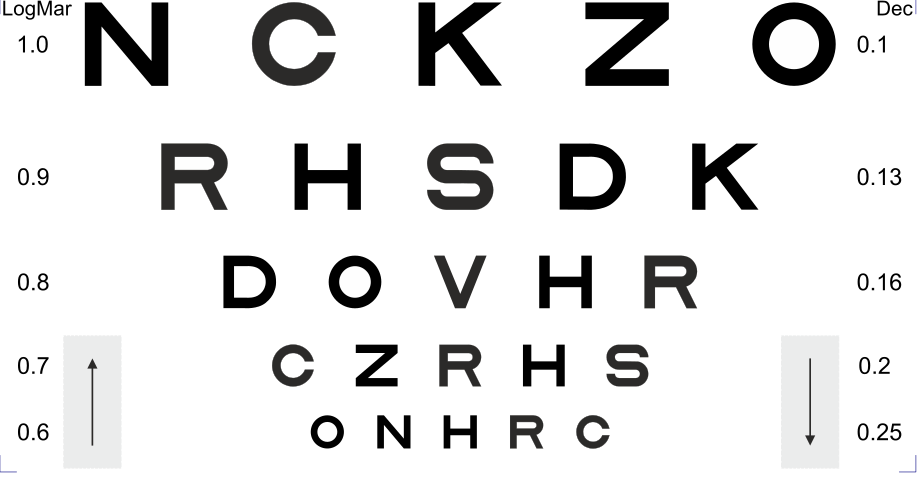
\includegraphics[width=.5\linewidth]{images/etdrs_top.png}
  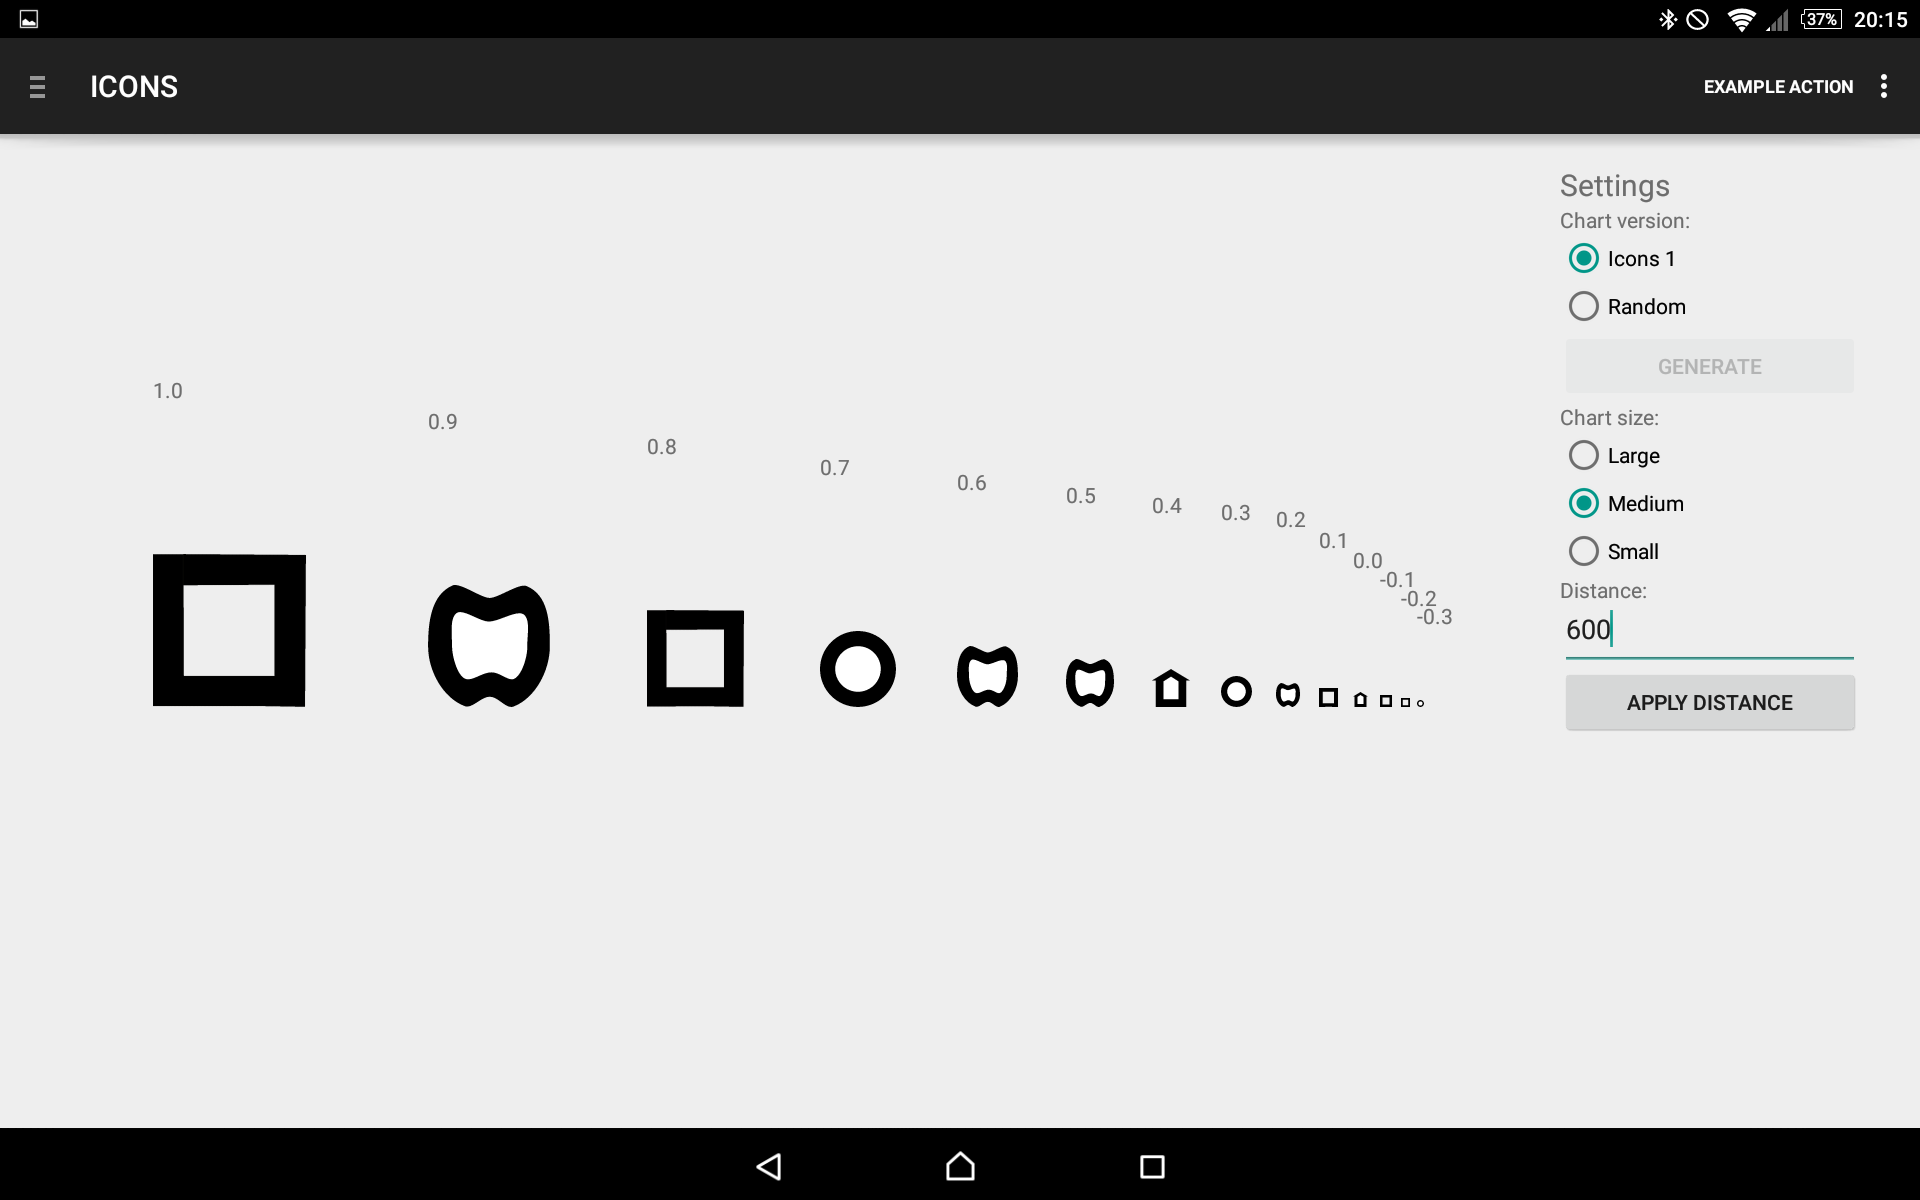
\includegraphics[width=60mm]{images/appgui/icons_medium.png}
  \caption{The medium Icons 1 chart}
  \label{fig:icons_medium}
\end{subfigure}%
\begin{subfigure}{.5\textwidth}
  \centering
  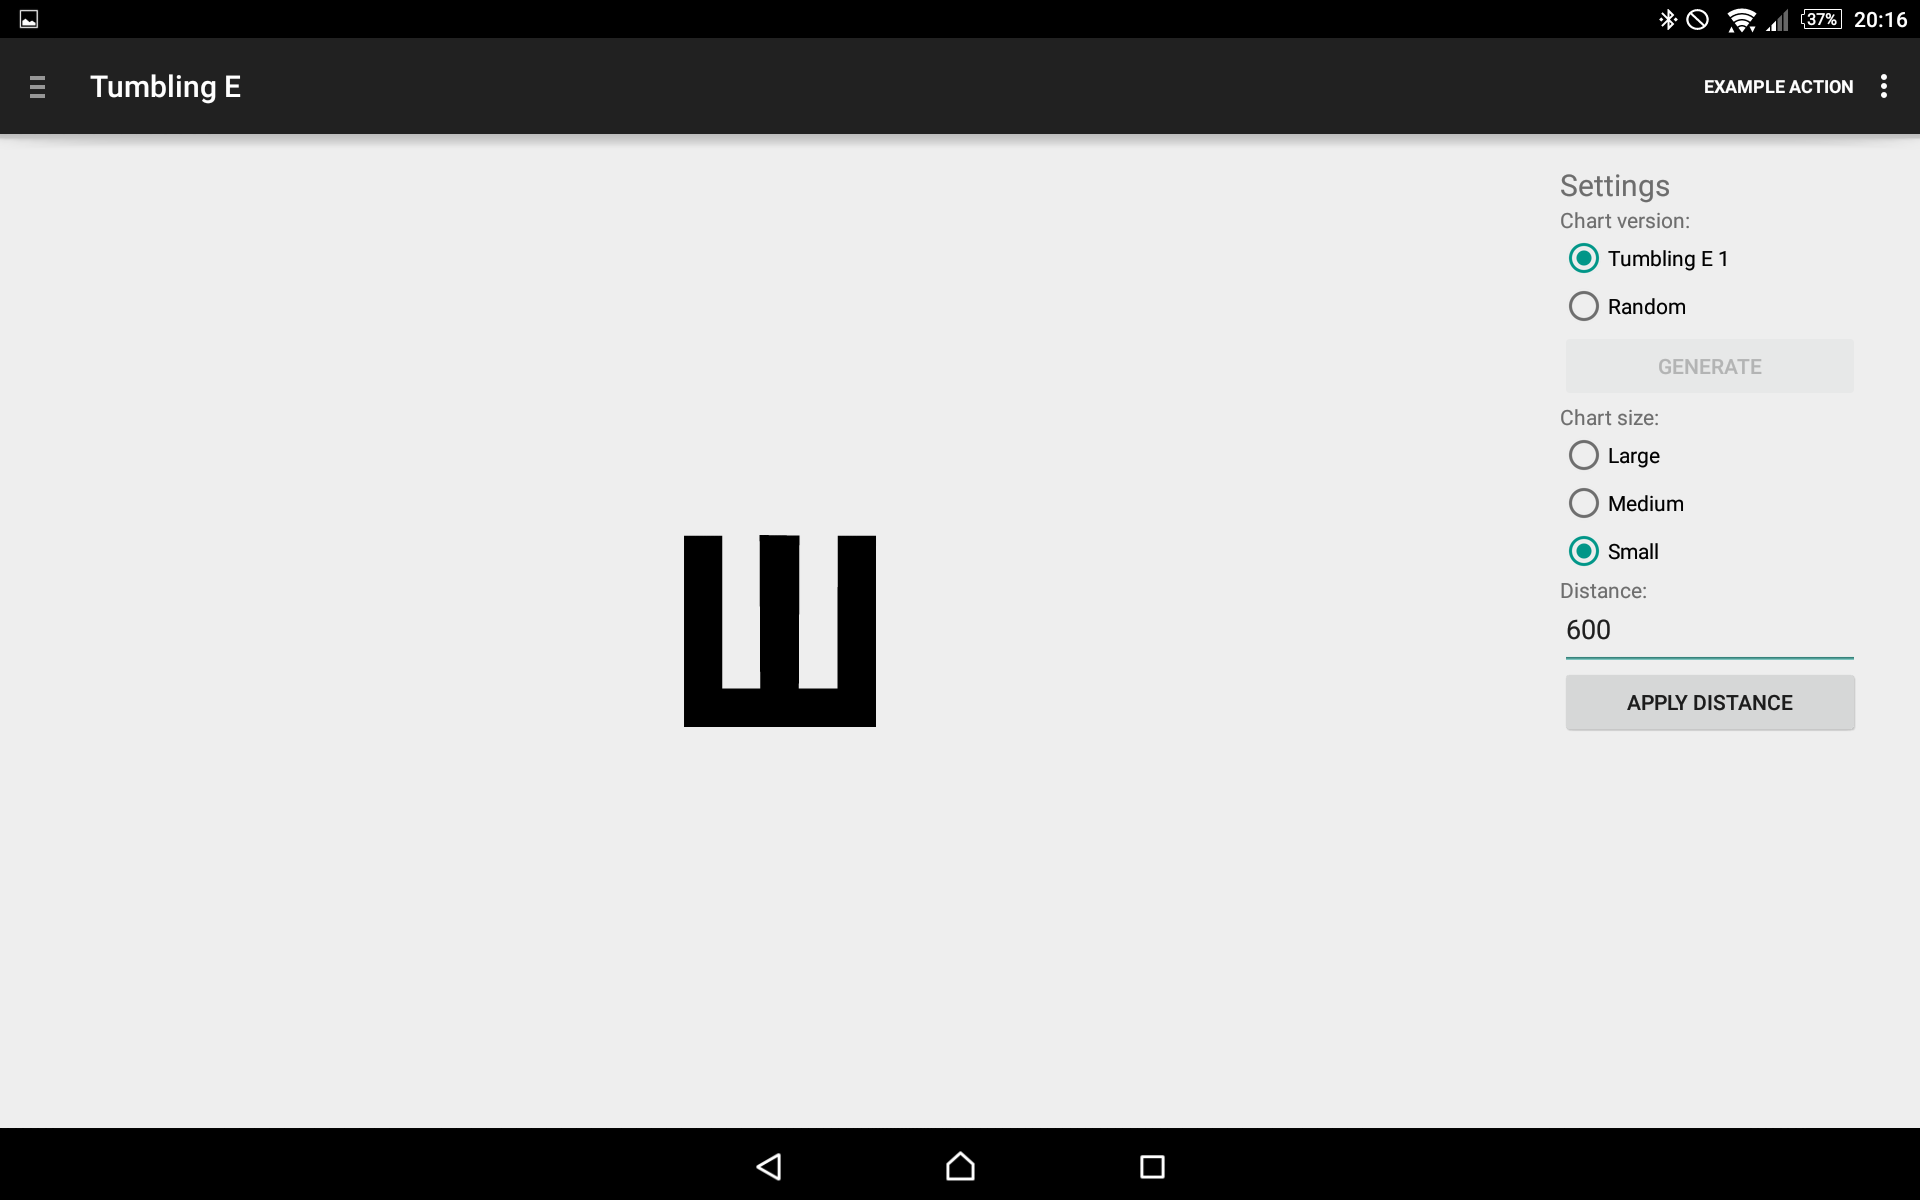
\includegraphics[width=60mm]{images/appgui/tumbling_e_small.png}
  \caption{The small Tumbling E 1 chart}
  \label{fig:tumbling_e_small}
\end{subfigure}
\caption{A medium and small chart}
\label{fig:chart_medium_small}
\end{figure}

The last setting the user can choose is the distance setting. Here the user can enter the distance a patient is from the screen, in centimeters, and then press \textit{Apply Distance}. This has no visible effect on the application but is used to set the optotype sizes on the monitor.

\subsection{Server}
The server application is in many ways very similar to the Android application. Both use the same methods for the calculations, such as the optotype sizes. The charts are built using the same code as the Android application with minor changes due to the fact that Java's Swing components have to be drawn rather than Android components. The monitor connected to the server only displays the currently chosen chart (fig. \ref{fig:server_charts}) and nothing else, such as LogMAR values or settings shown on the Android device.

\begin{figure}[ht!]
\centering
\begin{subfigure}{.5\textwidth}
  \centering
  %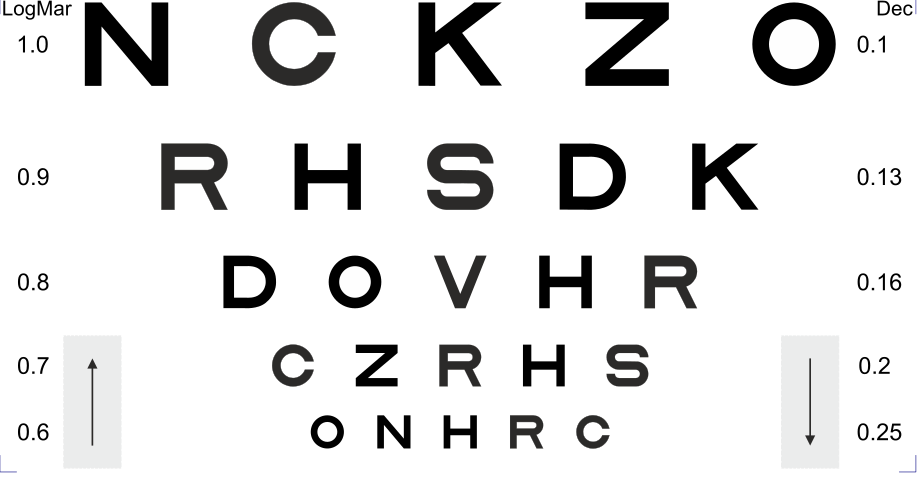
\includegraphics[width=.5\linewidth]{images/etdrs_top.png}
  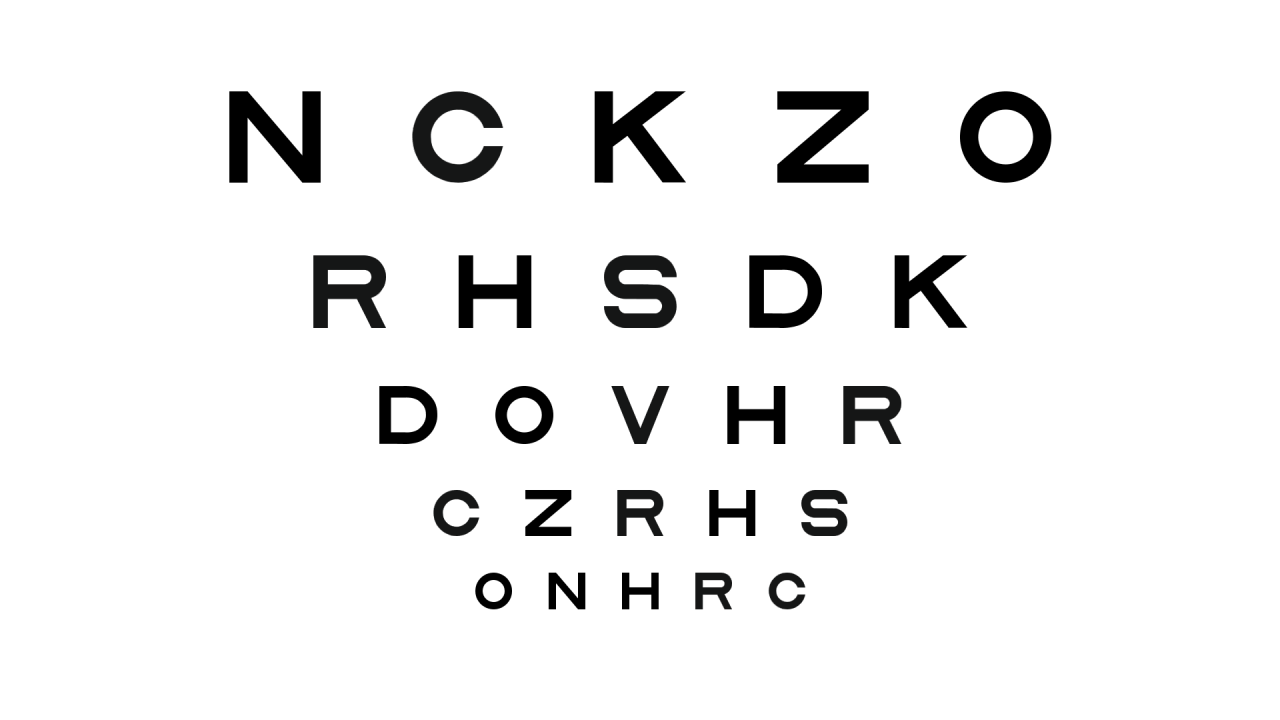
\includegraphics[width=60mm]{images/servergui/etdrs_chart.png}
  \caption{The large ETDRS chart}
  \label{fig:server_large}
\end{subfigure}%
\begin{subfigure}{.5\textwidth}
  \centering
  
\includegraphics[width=60mm]{images/servergui/etdrs_single_row.png}
  \caption{The medium ETDRS chart}
  \label{fig:server_medium}
\end{subfigure}
\caption{Example of charts as shown on the monitor connected to the server}
\label{fig:server_charts}
\end{figure}

\subsection{Known bugs and issues}
Even though the system fulfills the requirements, it doesn't mean it's bug free. If the network is unstable or slow, the server can react several seconds later than the Android application. This can cause a user to repeat an action which will, in the end, result in the server acting on on both actions. In the case that the connection gets broken, all actions performed will be ignored by the server, even after reconnecting. In this case, the user can change to another chart size or version and then back again to resolve the issue.

\section{Tests}
The four tests presented in section \ref{sec:evaluation} were performed in order to find major faults with the system. All tests is considered to have met the requirements, though the usability could still use some improvements.

\subsection{Developer walkthrough}
During the developer walkthrough of the system, all charts versions were found and all settings were usable on every chart by using table \ref{tab:test1}. The connection settings were also reachable from everywhere in the application and both connecting and reconnecting was working properly.

\begin{table}[ht!]
\centering
\begin{tabular}{l c c c r}
Chart version		&	Large		&	Medium		&	Small		&	Distance	\\
\hline\hline
ETDRS 1				&	\checkmark	&	\checkmark	&	\checkmark	&	\checkmark	\\
ETDRS 2				&	\checkmark	&	\checkmark	&	\checkmark	&	\checkmark	\\
ETDRS R				&	\checkmark	&	\checkmark	&	\checkmark	&	\checkmark	\\
ETDRS Random		&	\checkmark	&	\checkmark	&	\checkmark	&	\checkmark	\\
\hline
Tumbling E 1		&	\checkmark	&	\checkmark	&	\checkmark	&	\checkmark	\\
Tumbling E Random	&	\checkmark	&	\checkmark	&	\checkmark	&	\checkmark	\\
\hline
HVOT 1				&	\checkmark	&	\checkmark	&	\checkmark	&	\checkmark	\\
HVOT Random			&	\checkmark	&	\checkmark	&	\checkmark	&	\checkmark	\\
\hline
Icons 1				&	\checkmark	&	\checkmark	&	\checkmark	&	\checkmark	\\
Icons Random		&	\checkmark	&	\checkmark	&	\checkmark	&	\checkmark	\\
\hline\hline
					&	Scanning	&	Connecting	& 	Reconnecting	& \\
Connection			&	\checkmark	&	\checkmark	&	\checkmark	&	\\
\hline\hline
\end{tabular}
\caption{Result of the developer walkthrough. \label{tab:test1}}
\end{table}

\newpage
\subsection{Optotype Sizes}
The optotype sizes were calculated for and measured on a 15.6 inch computer screen and a 37 inch TV, both with 1920x1080 resolution. As the TV is larger than the computer screen, and have the same resolution, each pixel is bigger and thus, the calculated size in pixels is smaller (table. \ref{tab:optotype_test}). The height in centimeters, rounded to two decimals, are both equal to the expected height and the test is considered successful.


\begin{table}[ht!]
\centering
\begin{tabular}{ p{1cm}|p{1cm}p{1cm}|p{1cm}p{1cm}|p{1cm} }
	 &	\multicolumn{2}{c}{\parbox{2cm}{\centering 15.6", 1920x1080}} & \multicolumn{2}{c}{\parbox{2cm}{\centering 37", 1920x1080}}	& 	Expected	\\
\hline
	 row  & px & cm & px & cm & cm \\
\hline\hline				
								1	&	162	&	2.91	&	68	&	2.91	&	2.91\\	
								2	&	128 & 	2.31	& 	54	&	2.31	&	2.31\\
		 						3	&	102 & 	1.84	& 	43	&	1.84	&	1.84\\
								4	&	81 	& 	1.46	& 	34	&	1.46	&	1.46\\
								5	&	64 	& 	1.16	& 	27	&	1.16	&	1.16\\
								6	&	51 	& 	0.92	& 	22	&	0.92	&	0.92\\
								7	&	41 	& 	0.73	& 	17	&	0.73	&	0.73\\
								8	&	32 	& 	0.58	& 	14	&	0.58	&	0.58\\
								9	&	26 	& 	0.46	& 	11	&	0.46	&	0.46\\
								10	&	20 	& 	0.37	& 	9	&	0.37	&	0.37\\
								11	&	16 	& 	0.29	& 	7	&	0.29	&	0.29\\
								12	&	13 	& 	0.23	& 	5	&	0.23	&	0.23\\
								13	&	10 	& 	0.18	& 	4	&	0.18	&	0.18\\
								14	&	8 	& 	0.15	& 	3	&	0.15	&	0.15\\
										\hline
\end{tabular}
\caption{Height of optotypes for a 15.6 and 37 inch screen, both with a 1920x1080 resolution. The rightmost column displays the expected height of the optotypes in cm} \label{tab:optotype_test}
\end{table}


\subsection{Usability}
The systems usability was tested with the help of two persons with no previous background related to visual acuity charts or eye examinations. After a brief explanation to the different types of charts they where asked to follow the procedures in \ref{app:usability}. Both persons had no problem performing any of the tasks with the exception of one of them didn't realize that you had to swipe the screen in order to switch between the upper and lower charts in the application.

\subsection{Server Detection}
The server detection test was done 3 times on a stable WiFi network. According to the results (Table. \ref{tab:server_detection_test}), every single one of the tests performed was successful in finding a server over 90\% of the time. The average success rate of the 3 tests was about 96.3\% which means that the server detection requirements are met.

\begin{table}[ht!]
\centering
\begin{tabular}{l c r}
Attempt	&	failures	&	succeses	\\
\hline
1	&	7	&	93	\\
2	&	1	&	99	\\
3	&	3	&	97	\\
\end{tabular}
\caption{The number of failures and successes during the server detection tests. \label{tab:server_detection_test}}
\end{table}

%\begin{figure}[ht!]
%\end{figure}

\chapter{ Conclusion}

\section{Discussion}
Even though the system turned out as intended, there is a lot left to do until it can be used clinically. First of all, the system must be tested for more bugs and unintended behavior. This should preferably be done by users other than the developers since the developers know how the system works and can't safely predict what another user will attempt to do. Then, after all found bugs have been removed, the system must be tested by experts in the field of ophthalmology in order to make sure that the built system actually is a valid solution. This will also give credibility to the system.

\section{Advantages of a digital system}
The advantages of a digital system is the ability to change the layout, optotypes and size of the chart without having to manually exchange charts. This will save both time and space as only one screen and a small Android device is necessary, while also providing easier access to specialized charts that will help patients with different needs. This system will also allow the visual acuity tests to take place in rooms that previously where too small, as the system will display optotypes at a size suitable for the distance the patient is from the monitor.

\section{Disadvantages of a digital system}
A disadvantage with this system is that digital screens become very expensive at large sizes, which limits the maximum distance a patient can sit from the screen. Another disadvantage is that the resolution, or rather pixel density, will limit how close to a screen a patient can sit without the optotypes looking pixelated. Pixel density is a measurement of how many pixels (dots) can fit in a small section of the screen, usually denoted as Pixels Per Inch (PPI) or Dots Per Inch (DPI). The higher the DPI is the better the quality of small details will be. This is very important when rendering type fonts because the edges should be as smooth as possible.

\section{Alternative solutions}
A possible alternative solution to a custom server running on a Raspberry Pi or other computer use a Chromecast instead. This could simplify the system for the user as this would make the Android application work similar to the many media streaming applications that exists today. Using a Chromecast would also make sure the user only have to worry about the Android application as the Chromecast is just a plug and play unit maintained by Google. The disadvantages to this is, as mentioned earlier, that an agreement with Google have to be signed. The application would also require an internet connection, opposed the the current system which only need a local network.

\section{Future Work}
Future work will include more charts and features for the system. One such feature is the grating acuity test, which allows testing of visual acuity on very young children or people with difficulties communicating \cite{PGSoderbergOral}. Another feature is to include the option to, instead of changing the size of the optotypes, change the LogMAR, so the top row doesn't necessarily start at 1.0 LogMAR. This will allow the chart to use the entire monitors screen no matter the distance from the patient to the screen.

Other charts to be included could be, for example, charts using the Landholt C, charts for testing color blindness or charts used for testing astigmatism. The random function for the charts should be improved, as it currently have no constraints whatsoever. These constraints would make sure that the same optotype, or to similar optotypes like \textit{C} and \textit{O}, won't be repeated to many times in a row.


%\bibliography{references}{}
\renewcommand\thechapter{ }
\bibliography{IEEEabrv,references}
%\bibliographystyle{ieeetr}
\bibliographystyle{IEEEtran}

\newpage
\appendix
\chapter{ Testing} \label{App:test}
\section{Developer walkthrough}
\begin{table}[ht!]
\centering
\begin{tabular}{l c c c r}
Chart version		&	Large		&	Medium		&	Small		&	Distance	\\
\hline\hline
ETDRS 1				&		&		&		&		\\
ETDRS 2				&		&		&		&		\\
ETDRS R				&		&		&		&		\\
ETDRS Random		&		&		&		&		\\
\hline
Tumbling E 1		&		&		&		&		\\
Tumbling E Random	&		&		&		&		\\
\hline
HVOT 1				&		&		&		&		\\
HVOT Random			&		&		&		&		\\
\hline
Icons 1				&		&		&		&		\\
Icons Random		&		&		&		&		\\
\hline\hline
			&	Scanning	&	Connecting	& Reconnecting	& \\
Connection	&	&	&	& \\
\hline\hline
\end{tabular}
%\label{tab:test1_empty}
\caption{\label{tab:test1_empty}}
\end{table}

\newpage
\section{Usability test procedure \label{app:usability}}
\begin{enumerate}\bfseries

\item Start application

\item Connect to server

\item Display ETDRS 1 Large upper chart with a distance of 2 meters

\item Display ETDRS 1 Large lower chart with a distance of 2 meters

\item Display HVOT Random chart medium with a distance of 1.7 meters

\item Generate a new HVOT chart

\item Display Icons 1 small chart with a distance of 1.5 meters

\item Page through Icons 1 small chart with a distance of 1.5 meters

\item Reconnect to server

\end{enumerate}
\end{document}
